\documentclass{book}
\usepackage[a4paper,top=2.5cm,bottom=2.5cm,left=2.5cm,right=2.5cm]{geometry}
\usepackage{makeidx}
\usepackage{natbib}
\usepackage{graphicx}
\usepackage{multicol}
\usepackage{float}
\usepackage{listings}
\usepackage{color}
\usepackage{ifthen}
\usepackage[table]{xcolor}
\usepackage{textcomp}
\usepackage{alltt}
\usepackage{ifpdf}
\ifpdf
\usepackage[pdftex,
            pagebackref=true,
            colorlinks=true,
            linkcolor=blue,
            unicode
           ]{hyperref}
\else
\usepackage[ps2pdf,
            pagebackref=true,
            colorlinks=true,
            linkcolor=blue,
            unicode
           ]{hyperref}
\usepackage{pspicture}
\fi
\usepackage[utf8]{inputenc}
\usepackage{mathptmx}
\usepackage[scaled=.90]{helvet}
\usepackage{courier}
\usepackage{sectsty}
\usepackage{amssymb}
\usepackage[titles]{tocloft}
\usepackage{doxygen}
\lstset{language=C++,inputencoding=utf8,basicstyle=\footnotesize,breaklines=true,breakatwhitespace=true,tabsize=4,numbers=left }
\makeindex
\setcounter{tocdepth}{3}
\renewcommand{\footrulewidth}{0.4pt}
\renewcommand{\familydefault}{\sfdefault}
\hfuzz=15pt
\setlength{\emergencystretch}{15pt}
\hbadness=750
\tolerance=750
\begin{document}
\hypersetup{pageanchor=false,citecolor=blue}
\begin{titlepage}
\vspace*{7cm}
\begin{center}
{\Large Seq\-D\-P\-T }\\
\vspace*{1cm}
{\large Generated by Doxygen 1.8.3.1}\\
\vspace*{0.5cm}
{\small Fri May 24 2013 01:08:46}\\
\end{center}
\end{titlepage}
\clearemptydoublepage
\pagenumbering{roman}
\tableofcontents
\clearemptydoublepage
\pagenumbering{arabic}
\hypersetup{pageanchor=true,citecolor=blue}
\chapter{Hierarchical Index}
\section{Class Hierarchy}
This inheritance list is sorted roughly, but not completely, alphabetically\-:\begin{DoxyCompactList}
\item \contentsline{section}{seqan\-:\-:Adapter\-Scoring\-Matrix}{\pageref{structseqan_1_1_adapter_scoring_matrix}}{}
\item \contentsline{section}{Adapter\-Trimming\-Params}{\pageref{struct_adapter_trimming_params}}{}
\item \contentsline{section}{Adapter\-Trimming\-Stats}{\pageref{struct_adapter_trimming_stats}}{}
\item \contentsline{section}{B\-W\-A}{\pageref{struct_b_w_a}}{}
\item \contentsline{section}{Demultiplexing\-Params}{\pageref{struct_demultiplexing_params}}{}
\item \contentsline{section}{Demultiplex\-Stats}{\pageref{struct_demultiplex_stats}}{}
\item \contentsline{section}{Dna5\-Q\-Adapter}{\pageref{struct_dna5_q_adapter}}{}
\item \contentsline{section}{Mean}{\pageref{struct_mean}}{}
\item \contentsline{section}{Mode}{\pageref{struct_mode}}{}
\begin{DoxyCompactList}
\item \contentsline{section}{Auto}{\pageref{struct_auto}}{}
\item \contentsline{section}{User}{\pageref{struct_user}}{}
\end{DoxyCompactList}
\item \contentsline{section}{Output\-Streams}{\pageref{class_output_streams}}{}
\item \contentsline{section}{Program\-Params}{\pageref{struct_program_params}}{}
\item \contentsline{section}{Quality\-Trimming\-Params}{\pageref{struct_quality_trimming_params}}{}
\item \contentsline{section}{Quality\-Trimming\-Stats}{\pageref{struct_quality_trimming_stats}}{}
\item \contentsline{section}{seqan\-:\-:Scoring\-Matrix\-Data\-\_\-$<$ int, Dna5, Adapter\-Scoring\-Matrix $>$}{\pageref{structseqan_1_1_scoring_matrix_data___3_01int_00_01_dna5_00_01_adapter_scoring_matrix_01_4}}{}
\item \contentsline{section}{S\-T\-R\-I\-N\-G\-\_\-\-R\-E\-V\-E\-R\-S\-E\-\_\-\-C\-O\-M\-P\-L\-E\-M\-E\-N\-T$<$ T\-Value $>$}{\pageref{struct_s_t_r_i_n_g___r_e_v_e_r_s_e___c_o_m_p_l_e_m_e_n_t}}{}
\item \contentsline{section}{Tail}{\pageref{struct_tail}}{}
\end{DoxyCompactList}

\chapter{Class Index}
\section{\-Class \-List}
\-Here are the classes, structs, unions and interfaces with brief descriptions\-:\begin{DoxyCompactList}
\item\contentsline{section}{\hyperlink{structseqan_1_1_g_fasta_record}{seqan\-::\-G\-Fasta\-Record$<$ T\-Sequence $>$} }{\pageref{structseqan_1_1_g_fasta_record}}{}
\item\contentsline{section}{\hyperlink{structseqan_1_1_g_match}{seqan\-::\-G\-Match$<$ T\-Score, T\-Sequence $>$} }{\pageref{structseqan_1_1_g_match}}{}
\item\contentsline{section}{\hyperlink{structseqan_1_1_g_score_storage}{seqan\-::\-G\-Score\-Storage$<$ T\-Score $>$} }{\pageref{structseqan_1_1_g_score_storage}}{}
\item\contentsline{section}{\hyperlink{structseqan_1_1_memory_sample}{seqan\-::\-Memory\-Sample} }{\pageref{structseqan_1_1_memory_sample}}{}
\item\contentsline{section}{\hyperlink{structseqan_1_1_performance_sample}{seqan\-::\-Performance\-Sample} }{\pageref{structseqan_1_1_performance_sample}}{}
\end{DoxyCompactList}

\chapter{File Index}
\section{File List}
Here is a list of all files with brief descriptions\-:\begin{DoxyCompactList}
\item\contentsline{section}{apps/\-G\-Benchmark/\hyperlink{_g_benchmark_8cpp}{G\-Benchmark.\-cpp} }{\pageref{_g_benchmark_8cpp}}{}
\item\contentsline{section}{apps/\-G\-Cluster/\hyperlink{_g_cluster_8cpp}{G\-Cluster.\-cpp} }{\pageref{_g_cluster_8cpp}}{}
\item\contentsline{section}{apps/\-G\-Search/\hyperlink{_g_search_8cpp}{G\-Search.\-cpp} }{\pageref{_g_search_8cpp}}{}
\item\contentsline{section}{include/seqan/\hyperlink{compare_files_8h}{compare\-Files.\-h} }{\pageref{compare_files_8h}}{}
\item\contentsline{section}{include/seqan/\hyperlink{compute_sens_spec_8h}{compute\-Sens\-Spec.\-h} }{\pageref{compute_sens_spec_8h}}{}
\item\contentsline{section}{include/seqan/\hyperlink{_g_cluster_8h}{G\-Cluster.\-h} }{\pageref{_g_cluster_8h}}{}
\item\contentsline{section}{include/seqan/\hyperlink{get_id_without_master_8h}{get\-Id\-Without\-Master.\-h} }{\pageref{get_id_without_master_8h}}{}
\item\contentsline{section}{include/seqan/\hyperlink{_g_search_8h}{G\-Search.\-h} }{\pageref{_g_search_8h}}{}
\item\contentsline{section}{include/seqan/\hyperlink{_g_structs_8h}{G\-Structs.\-h} }{\pageref{_g_structs_8h}}{}
\item\contentsline{section}{include/seqan/\-G\-Cluster/\hyperlink{_g_assign_cluster_8h}{G\-Assign\-Cluster.\-h} }{\pageref{_g_assign_cluster_8h}}{}
\item\contentsline{section}{include/seqan/\-G\-Cluster/\hyperlink{_g_check_cluster_assign_8h}{G\-Check\-Cluster\-Assign.\-h} }{\pageref{_g_check_cluster_assign_8h}}{}
\item\contentsline{section}{include/seqan/\-G\-Cluster/\hyperlink{_g_cluster__base_8h}{G\-Cluster\-\_\-base.\-h} }{\pageref{_g_cluster__base_8h}}{}
\item\contentsline{section}{include/seqan/\-G\-Search/\hyperlink{_g_check_cluster_master_8h}{G\-Check\-Cluster\-Master.\-h} }{\pageref{_g_check_cluster_master_8h}}{}
\item\contentsline{section}{include/seqan/\-G\-Search/\hyperlink{_g_compute_match_8h}{G\-Compute\-Match.\-h} }{\pageref{_g_compute_match_8h}}{}
\item\contentsline{section}{include/seqan/\-G\-Search/\hyperlink{_g_evaluate_score_8h}{G\-Evaluate\-Score.\-h} }{\pageref{_g_evaluate_score_8h}}{}
\item\contentsline{section}{include/seqan/\-G\-Search/\hyperlink{_g_parse_master_id_8h}{G\-Parse\-Master\-Id.\-h} }{\pageref{_g_parse_master_id_8h}}{}
\item\contentsline{section}{include/seqan/\-G\-Search/\hyperlink{_g_post_process_matches_8h}{G\-Post\-Process\-Matches.\-h} }{\pageref{_g_post_process_matches_8h}}{}
\item\contentsline{section}{include/seqan/\-G\-Search/\hyperlink{_g_score_8h}{G\-Score.\-h} }{\pageref{_g_score_8h}}{}
\item\contentsline{section}{include/seqan/\-G\-Search/\hyperlink{_g_score_peptide_q_gram_8h}{G\-Score\-Peptide\-Q\-Gram.\-h} }{\pageref{_g_score_peptide_q_gram_8h}}{}
\item\contentsline{section}{include/seqan/\-G\-Search/\hyperlink{_g_search__base_8h}{G\-Search\-\_\-base.\-h} }{\pageref{_g_search__base_8h}}{}
\item\contentsline{section}{include/seqan/\-G\-Search/\hyperlink{_g_write_matches_8h}{G\-Write\-Matches.\-h} }{\pageref{_g_write_matches_8h}}{}
\item\contentsline{section}{include/seqan/\-G\-Structs/\hyperlink{_g_fasta_record_8h}{G\-Fasta\-Record.\-h} }{\pageref{_g_fasta_record_8h}}{}
\item\contentsline{section}{include/seqan/\-G\-Structs/\hyperlink{_g_match_8h}{G\-Match.\-h} }{\pageref{_g_match_8h}}{}
\item\contentsline{section}{include/seqan/\-G\-Structs/\hyperlink{_g_score_storage_8h}{G\-Score\-Storage.\-h} }{\pageref{_g_score_storage_8h}}{}
\item\contentsline{section}{include/seqan/\-G\-Structs/\hyperlink{_memory_sample_8h}{Memory\-Sample.\-h} }{\pageref{_memory_sample_8h}}{}
\item\contentsline{section}{include/seqan/\-G\-Structs/\hyperlink{_performance_sample_8h}{Performance\-Sample.\-h} }{\pageref{_performance_sample_8h}}{}
\item\contentsline{section}{tests/\-G\-Cluster/\hyperlink{test___g_assign_cluster_8h}{test\-\_\-\-G\-Assign\-Cluster.\-h} }{\pageref{test___g_assign_cluster_8h}}{}
\item\contentsline{section}{tests/\-G\-Cluster/\hyperlink{test___g_check_cluster_assign_8h}{test\-\_\-\-G\-Check\-Cluster\-Assign.\-h} }{\pageref{test___g_check_cluster_assign_8h}}{}
\item\contentsline{section}{tests/\-G\-Cluster/\hyperlink{test___g_cluster_8cpp}{test\-\_\-\-G\-Cluster.\-cpp} }{\pageref{test___g_cluster_8cpp}}{}
\item\contentsline{section}{tests/\-G\-Cluster/\hyperlink{test___g_cluster__system_test_8h}{test\-\_\-\-G\-Cluster\-\_\-system\-Test.\-h} }{\pageref{test___g_cluster__system_test_8h}}{}
\item\contentsline{section}{tests/\-G\-Search/\hyperlink{test___g_check_cluster_master_8h}{test\-\_\-\-G\-Check\-Cluster\-Master.\-h} }{\pageref{test___g_check_cluster_master_8h}}{}
\item\contentsline{section}{tests/\-G\-Search/\hyperlink{test___g_compute_match_8h}{test\-\_\-\-G\-Compute\-Match.\-h} }{\pageref{test___g_compute_match_8h}}{}
\item\contentsline{section}{tests/\-G\-Search/\hyperlink{test___g_evaluate_score_8h}{test\-\_\-\-G\-Evaluate\-Score.\-h} }{\pageref{test___g_evaluate_score_8h}}{}
\item\contentsline{section}{tests/\-G\-Search/\hyperlink{test___g_parse_master_id_8h}{test\-\_\-\-G\-Parse\-Master\-Id.\-h} }{\pageref{test___g_parse_master_id_8h}}{}
\item\contentsline{section}{tests/\-G\-Search/\hyperlink{test___g_post_process_matches_8h}{test\-\_\-\-G\-Post\-Process\-Matches.\-h} }{\pageref{test___g_post_process_matches_8h}}{}
\item\contentsline{section}{tests/\-G\-Search/\hyperlink{test___g_score_8h}{test\-\_\-\-G\-Score.\-h} }{\pageref{test___g_score_8h}}{}
\item\contentsline{section}{tests/\-G\-Search/\hyperlink{test___g_score_peptide_q_gram_8h}{test\-\_\-\-G\-Score\-Peptide\-Q\-Gram.\-h} }{\pageref{test___g_score_peptide_q_gram_8h}}{}
\item\contentsline{section}{tests/\-G\-Search/\hyperlink{test___g_search_8cpp}{test\-\_\-\-G\-Search.\-cpp} }{\pageref{test___g_search_8cpp}}{}
\item\contentsline{section}{tests/\-G\-Search/\hyperlink{test___g_search__system_test_8h}{test\-\_\-\-G\-Search\-\_\-system\-Test.\-h} }{\pageref{test___g_search__system_test_8h}}{}
\item\contentsline{section}{tests/\-G\-Search/\hyperlink{test___g_write_matches_8h}{test\-\_\-\-G\-Write\-Matches.\-h} }{\pageref{test___g_write_matches_8h}}{}
\end{DoxyCompactList}

\chapter{Class Documentation}
\hypertarget{structseqan_1_1_adapter_scoring_matrix}{\section{seqan\-:\-:Adapter\-Scoring\-Matrix Struct Reference}
\label{structseqan_1_1_adapter_scoring_matrix}\index{seqan\-::\-Adapter\-Scoring\-Matrix@{seqan\-::\-Adapter\-Scoring\-Matrix}}
}


Struct used to define a new custom scoring matrix.  




{\ttfamily \#include $<$adapter\-Trimming.\-h$>$}



\subsection{Detailed Description}
Struct used to define a new custom scoring matrix. 

The documentation for this struct was generated from the following file\-:\begin{DoxyCompactItemize}
\item 
D\-:/\-Seq\-An/\-Development/seqan-\/trunk/sandbox/my\-\_\-sandbox/apps/\-Seq\-D\-P\-T/\hyperlink{adapter_trimming_8h}{adapter\-Trimming.\-h}\end{DoxyCompactItemize}

\hypertarget{struct_adapter_trimming_params}{\section{Adapter\-Trimming\-Params Struct Reference}
\label{struct_adapter_trimming_params}\index{Adapter\-Trimming\-Params@{Adapter\-Trimming\-Params}}
}


Struct holding all adapter trimming parameters.  


\subsection*{Public Attributes}
\begin{DoxyCompactItemize}
\item 
bool \hyperlink{struct_adapter_trimming_params_a9c442bd3226e26f0becce6eba5f40359}{paired}
\item 
bool \hyperlink{struct_adapter_trimming_params_a8386f1819859d97bb58011903f5dd847}{no\-Adapter}
\item 
bool \hyperlink{struct_adapter_trimming_params_a61f37e8fe2d242947cfd358b85a0380e}{run}
\item 
Dna5\-Q\-String \hyperlink{struct_adapter_trimming_params_a2ce2d426a36e328f4fceb715910db488}{adapter1}
\item 
Dna5\-Q\-String \hyperlink{struct_adapter_trimming_params_aa7d555b99c145cd062e7caa12f4161ab}{adapter2}
\item 
\hyperlink{struct_mode}{Mode} \hyperlink{struct_adapter_trimming_params_a9e78ea3942b231eccb2243a70953c560}{mode}
\item 
Match\-Mode \hyperlink{struct_adapter_trimming_params_ae69ec37f149e6b9234746ae275c5ff3e}{mmode}
\item 
\hyperlink{struct_adapter_trimming_stats}{Adapter\-Trimming\-Stats} \hyperlink{struct_adapter_trimming_params_a557d501f056a0ba2ae35560ed8d72a9d}{stats}
\end{DoxyCompactItemize}


\subsection{Detailed Description}
Struct holding all adapter trimming parameters. 

Struct holding the parameters needed for adapter trimming. 

\subsection{Member Data Documentation}
\hypertarget{struct_adapter_trimming_params_a2ce2d426a36e328f4fceb715910db488}{\index{Adapter\-Trimming\-Params@{Adapter\-Trimming\-Params}!adapter1@{adapter1}}
\index{adapter1@{adapter1}!AdapterTrimmingParams@{Adapter\-Trimming\-Params}}
\subsubsection[{adapter1}]{\setlength{\rightskip}{0pt plus 5cm}Dna5\-Q\-String Adapter\-Trimming\-Params\-::adapter1}}\label{struct_adapter_trimming_params_a2ce2d426a36e328f4fceb715910db488}
Holds the first adapter. \hypertarget{struct_adapter_trimming_params_aa7d555b99c145cd062e7caa12f4161ab}{\index{Adapter\-Trimming\-Params@{Adapter\-Trimming\-Params}!adapter2@{adapter2}}
\index{adapter2@{adapter2}!AdapterTrimmingParams@{Adapter\-Trimming\-Params}}
\subsubsection[{adapter2}]{\setlength{\rightskip}{0pt plus 5cm}Dna5\-Q\-String Adapter\-Trimming\-Params\-::adapter2}}\label{struct_adapter_trimming_params_aa7d555b99c145cd062e7caa12f4161ab}
Holds the second adapter \hypertarget{struct_adapter_trimming_params_ae69ec37f149e6b9234746ae275c5ff3e}{\index{Adapter\-Trimming\-Params@{Adapter\-Trimming\-Params}!mmode@{mmode}}
\index{mmode@{mmode}!AdapterTrimmingParams@{Adapter\-Trimming\-Params}}
\subsubsection[{mmode}]{\setlength{\rightskip}{0pt plus 5cm}Match\-Mode Adapter\-Trimming\-Params\-::mmode}}\label{struct_adapter_trimming_params_ae69ec37f149e6b9234746ae275c5ff3e}
Enum, indicating which trimming mode is used. Necessary for casting mode. \hypertarget{struct_adapter_trimming_params_a9e78ea3942b231eccb2243a70953c560}{\index{Adapter\-Trimming\-Params@{Adapter\-Trimming\-Params}!mode@{mode}}
\index{mode@{mode}!AdapterTrimmingParams@{Adapter\-Trimming\-Params}}
\subsubsection[{mode}]{\setlength{\rightskip}{0pt plus 5cm}{\bf Mode} Adapter\-Trimming\-Params\-::mode}}\label{struct_adapter_trimming_params_a9e78ea3942b231eccb2243a70953c560}
Hold the \hyperlink{struct_mode}{Mode}-\/object which determines which trimming mode shall be used. \hypertarget{struct_adapter_trimming_params_a8386f1819859d97bb58011903f5dd847}{\index{Adapter\-Trimming\-Params@{Adapter\-Trimming\-Params}!no\-Adapter@{no\-Adapter}}
\index{no\-Adapter@{no\-Adapter}!AdapterTrimmingParams@{Adapter\-Trimming\-Params}}
\subsubsection[{no\-Adapter}]{\setlength{\rightskip}{0pt plus 5cm}bool Adapter\-Trimming\-Params\-::no\-Adapter}}\label{struct_adapter_trimming_params_a8386f1819859d97bb58011903f5dd847}
T\-R\-U\-E if no adapter file is provided. \hypertarget{struct_adapter_trimming_params_a9c442bd3226e26f0becce6eba5f40359}{\index{Adapter\-Trimming\-Params@{Adapter\-Trimming\-Params}!paired@{paired}}
\index{paired@{paired}!AdapterTrimmingParams@{Adapter\-Trimming\-Params}}
\subsubsection[{paired}]{\setlength{\rightskip}{0pt plus 5cm}bool Adapter\-Trimming\-Params\-::paired}}\label{struct_adapter_trimming_params_a9c442bd3226e26f0becce6eba5f40359}
T\-R\-U\-E if paired-\/end data is used. \hypertarget{struct_adapter_trimming_params_a61f37e8fe2d242947cfd358b85a0380e}{\index{Adapter\-Trimming\-Params@{Adapter\-Trimming\-Params}!run@{run}}
\index{run@{run}!AdapterTrimmingParams@{Adapter\-Trimming\-Params}}
\subsubsection[{run}]{\setlength{\rightskip}{0pt plus 5cm}bool Adapter\-Trimming\-Params\-::run}}\label{struct_adapter_trimming_params_a61f37e8fe2d242947cfd358b85a0380e}
T\-R\-U\-E if the adapter trimming shall be run. \hypertarget{struct_adapter_trimming_params_a557d501f056a0ba2ae35560ed8d72a9d}{\index{Adapter\-Trimming\-Params@{Adapter\-Trimming\-Params}!stats@{stats}}
\index{stats@{stats}!AdapterTrimmingParams@{Adapter\-Trimming\-Params}}
\subsubsection[{stats}]{\setlength{\rightskip}{0pt plus 5cm}{\bf Adapter\-Trimming\-Stats} Adapter\-Trimming\-Params\-::stats}}\label{struct_adapter_trimming_params_a557d501f056a0ba2ae35560ed8d72a9d}
Holds interesting numbers about trimmed adapters. 

The documentation for this struct was generated from the following file\-:\begin{DoxyCompactItemize}
\item 
D\-:/\-Seq\-An/\-Development/seqan-\/trunk/sandbox/my\-\_\-sandbox/apps/\-Seq\-D\-P\-T/Seq\-D\-P\-T.\-cpp\end{DoxyCompactItemize}

\hypertarget{struct_adapter_trimming_stats}{\section{Adapter\-Trimming\-Stats Struct Reference}
\label{struct_adapter_trimming_stats}\index{Adapter\-Trimming\-Stats@{Adapter\-Trimming\-Stats}}
}


Struct to hold information about certain adapter trimming statistics.  




{\ttfamily \#include $<$adapter\-Trimming.\-h$>$}

\subsection*{Public Member Functions}
\begin{DoxyCompactItemize}
\item 
\hypertarget{struct_adapter_trimming_stats_aba2db4f8bdfbf1f9d389bf20a752b8f3}{void {\bfseries clear} ()}\label{struct_adapter_trimming_stats_aba2db4f8bdfbf1f9d389bf20a752b8f3}

\end{DoxyCompactItemize}
\subsection*{Public Attributes}
\begin{DoxyCompactItemize}
\item 
\hypertarget{struct_adapter_trimming_stats_ac2e7c09b2e9b8a080afb148c6f8d4026}{unsigned {\bfseries a1count}}\label{struct_adapter_trimming_stats_ac2e7c09b2e9b8a080afb148c6f8d4026}

\item 
unsigned \hyperlink{struct_adapter_trimming_stats_aabec417e43e59c829ab9172399c2961f}{a2count}
\item 
unsigned \hyperlink{struct_adapter_trimming_stats_a1a223cef64dde7c1a3eb5f7a8da182b5}{overlap\-Sum}
\item 
\hypertarget{struct_adapter_trimming_stats_ac893758e439beec68892ce129b16bc82}{unsigned {\bfseries min\-Overlap}}\label{struct_adapter_trimming_stats_ac893758e439beec68892ce129b16bc82}

\item 
unsigned \hyperlink{struct_adapter_trimming_stats_a3a8e65c4bb3dbd65a51289d07699ad11}{max\-Overlap}
\end{DoxyCompactItemize}


\subsection{Detailed Description}
Struct to hold information about certain adapter trimming statistics. 

\subsection{Member Data Documentation}
\hypertarget{struct_adapter_trimming_stats_aabec417e43e59c829ab9172399c2961f}{\index{Adapter\-Trimming\-Stats@{Adapter\-Trimming\-Stats}!a2count@{a2count}}
\index{a2count@{a2count}!AdapterTrimmingStats@{Adapter\-Trimming\-Stats}}
\subsubsection[{a2count}]{\setlength{\rightskip}{0pt plus 5cm}unsigned Adapter\-Trimming\-Stats\-::a2count}}\label{struct_adapter_trimming_stats_aabec417e43e59c829ab9172399c2961f}
The number of adapters present in forward and backward reads. \hypertarget{struct_adapter_trimming_stats_a3a8e65c4bb3dbd65a51289d07699ad11}{\index{Adapter\-Trimming\-Stats@{Adapter\-Trimming\-Stats}!max\-Overlap@{max\-Overlap}}
\index{max\-Overlap@{max\-Overlap}!AdapterTrimmingStats@{Adapter\-Trimming\-Stats}}
\subsubsection[{max\-Overlap}]{\setlength{\rightskip}{0pt plus 5cm}unsigned Adapter\-Trimming\-Stats\-::max\-Overlap}}\label{struct_adapter_trimming_stats_a3a8e65c4bb3dbd65a51289d07699ad11}
Minimum and maximum overlap between adapter and reads. \hypertarget{struct_adapter_trimming_stats_a1a223cef64dde7c1a3eb5f7a8da182b5}{\index{Adapter\-Trimming\-Stats@{Adapter\-Trimming\-Stats}!overlap\-Sum@{overlap\-Sum}}
\index{overlap\-Sum@{overlap\-Sum}!AdapterTrimmingStats@{Adapter\-Trimming\-Stats}}
\subsubsection[{overlap\-Sum}]{\setlength{\rightskip}{0pt plus 5cm}unsigned Adapter\-Trimming\-Stats\-::overlap\-Sum}}\label{struct_adapter_trimming_stats_a1a223cef64dde7c1a3eb5f7a8da182b5}
The sum of the removed adapter bases. Later used to calculate mean adapter size. 

The documentation for this struct was generated from the following file\-:\begin{DoxyCompactItemize}
\item 
D\-:/\-Seq\-An/\-Development/seqan-\/trunk/sandbox/my\-\_\-sandbox/apps/\-Seq\-D\-P\-T/\hyperlink{adapter_trimming_8h}{adapter\-Trimming.\-h}\end{DoxyCompactItemize}

\hypertarget{struct_auto}{\section{Auto Struct Reference}
\label{struct_auto}\index{Auto@{Auto}}
}


Tagging struct for the automatic match algorithm.  




{\ttfamily \#include $<$adapter\-Trimming.\-h$>$}

Inheritance diagram for Auto\-:\begin{figure}[H]
\begin{center}
\leavevmode
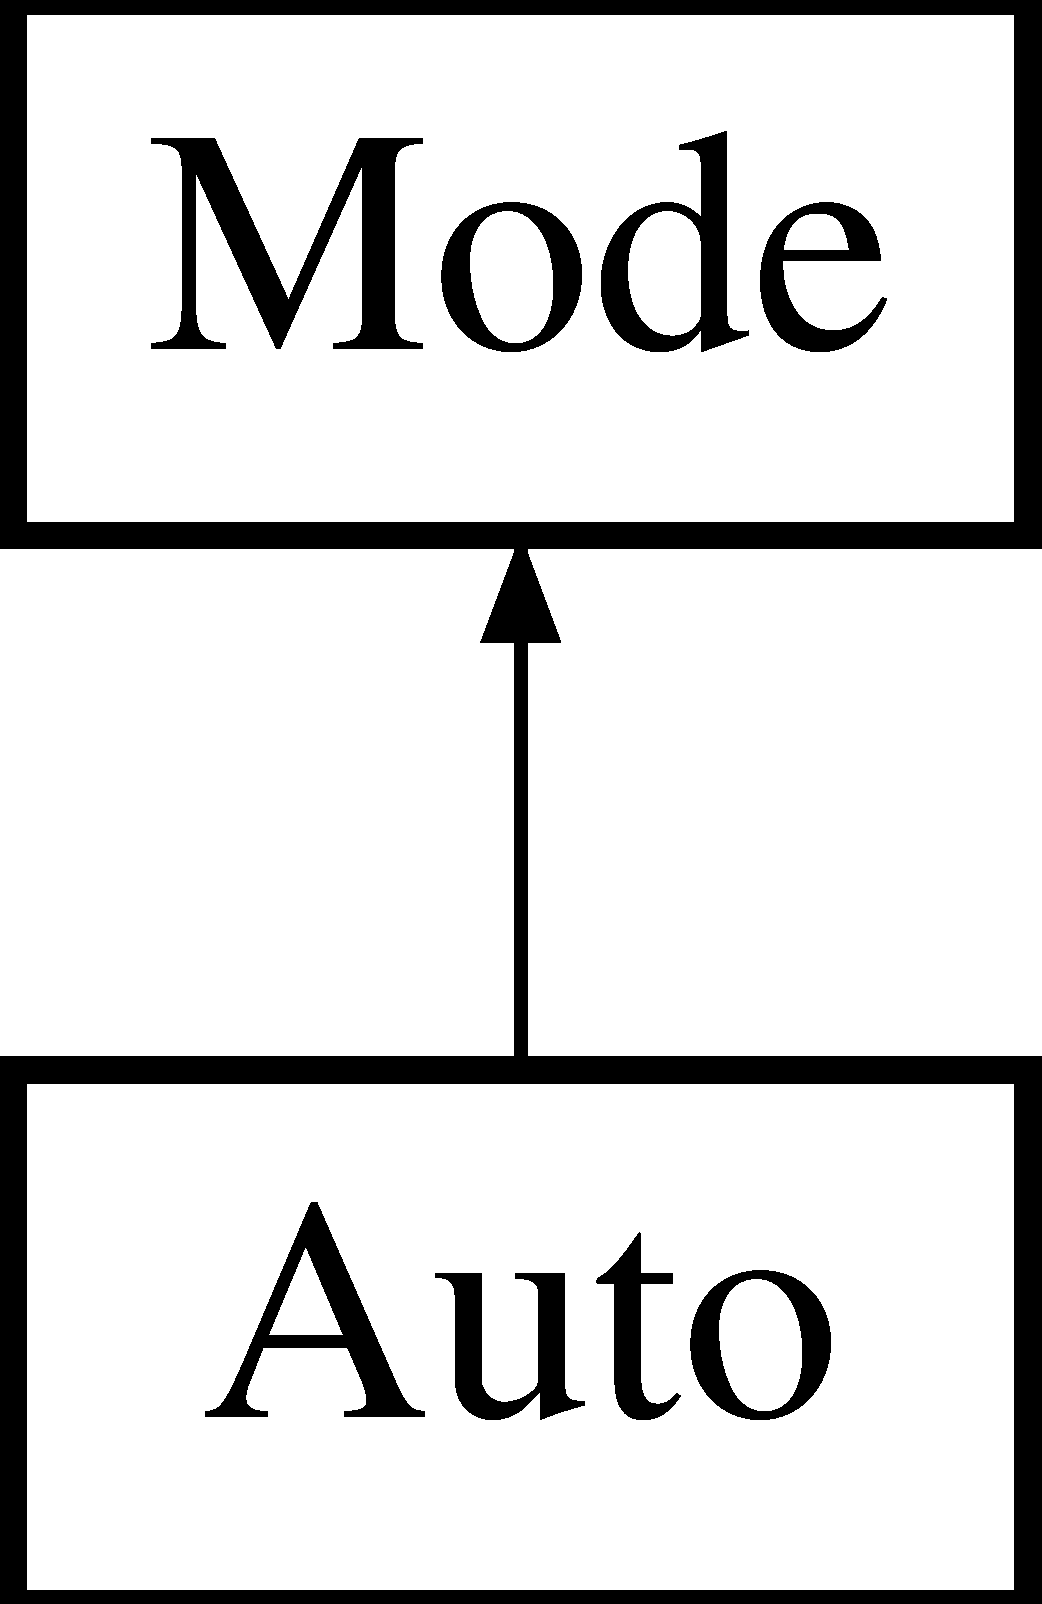
\includegraphics[height=2.000000cm]{struct_auto}
\end{center}
\end{figure}


\subsection{Detailed Description}
Tagging struct for the automatic match algorithm. 

The documentation for this struct was generated from the following file\-:\begin{DoxyCompactItemize}
\item 
D\-:/\-Seq\-An/\-Development/seqan-\/trunk/sandbox/my\-\_\-sandbox/apps/\-Seq\-D\-P\-T/\hyperlink{adapter_trimming_8h}{adapter\-Trimming.\-h}\end{DoxyCompactItemize}

\hypertarget{struct_b_w_a}{\section{B\-W\-A Struct Reference}
\label{struct_b_w_a}\index{B\-W\-A@{B\-W\-A}}
}


The tagging structure for the \hyperlink{struct_b_w_a}{B\-W\-A} trimming algorithm.  




{\ttfamily \#include $<$read\-Trimming.\-h$>$}



\subsection{Detailed Description}
The tagging structure for the \hyperlink{struct_b_w_a}{B\-W\-A} trimming algorithm. 

The documentation for this struct was generated from the following file\-:\begin{DoxyCompactItemize}
\item 
D\-:/\-Seq\-An/\-Development/seqan-\/trunk/sandbox/my\-\_\-sandbox/apps/\-Seq\-D\-P\-T/\hyperlink{read_trimming_8h}{read\-Trimming.\-h}\end{DoxyCompactItemize}

\hypertarget{struct_demultiplexing_params}{\section{Demultiplexing\-Params Struct Reference}
\label{struct_demultiplexing_params}\index{Demultiplexing\-Params@{Demultiplexing\-Params}}
}


Struct holding all demultiplexing parameters.  


\subsection*{Public Attributes}
\begin{DoxyCompactItemize}
\item 
seqan\-::\-String$<$ char $>$ \hyperlink{struct_demultiplexing_params_a2b2b682fbf21f3ca8daafe3e9b83c0ca}{barcode\-File}
\item 
seqan\-::\-String\-Set\\*
$<$ seqan\-::\-String$<$ seqan\-::\-Dna $>$ $>$ \hyperlink{struct_demultiplexing_params_aaeea114c00f19f6565047e507a74f90f}{barcodes}
\item 
seqan\-::\-String\-Set\\*
$<$ seqan\-::\-String$<$ char $>$ $>$ \hyperlink{struct_demultiplexing_params_a1721fa9ad83112b0d2df9c2932bd00be}{barcode\-Ids}
\item 
seqan\-::\-String$<$ char $>$ \hyperlink{struct_demultiplexing_params_a93d9e02c35225dac383b7c52f7b539f7}{multiplex\-File}
\item 
seqan\-::\-String\-Set\\*
$<$ seqan\-::\-String$<$ seqan\-::\-Dna5\-Q $>$ $>$ \hyperlink{struct_demultiplexing_params_a6d5a685bccab390519e4b423018443f7}{multiplex}
\item 
bool \hyperlink{struct_demultiplexing_params_ae76872bea7b75ea020035f7825fc8210}{approximate}
\item 
bool \hyperlink{struct_demultiplexing_params_a28920791fd2dfa590dade23f2924b93a}{hard\-Clip}
\item 
bool \hyperlink{struct_demultiplexing_params_a4a52e0b0dbbacf3e1d4e2b115f3d8cf7}{run}
\item 
bool \hyperlink{struct_demultiplexing_params_aa7bf93a371b34c9ad7ae0a5dc8edc8c5}{runx}
\item 
\hyperlink{struct_demultiplex_stats}{Demultiplex\-Stats} \hyperlink{struct_demultiplexing_params_a1017a69229d12a8a3714f80e75c3dbb9}{stats}
\end{DoxyCompactItemize}


\subsection{Detailed Description}
Struct holding all demultiplexing parameters. 

\subsection{Member Data Documentation}
\hypertarget{struct_demultiplexing_params_ae76872bea7b75ea020035f7825fc8210}{\index{Demultiplexing\-Params@{Demultiplexing\-Params}!approximate@{approximate}}
\index{approximate@{approximate}!DemultiplexingParams@{Demultiplexing\-Params}}
\subsubsection[{approximate}]{\setlength{\rightskip}{0pt plus 5cm}bool Demultiplexing\-Params\-::approximate}}\label{struct_demultiplexing_params_ae76872bea7b75ea020035f7825fc8210}
T\-R\-U\-E if approximate search shall be used \hypertarget{struct_demultiplexing_params_a2b2b682fbf21f3ca8daafe3e9b83c0ca}{\index{Demultiplexing\-Params@{Demultiplexing\-Params}!barcode\-File@{barcode\-File}}
\index{barcode\-File@{barcode\-File}!DemultiplexingParams@{Demultiplexing\-Params}}
\subsubsection[{barcode\-File}]{\setlength{\rightskip}{0pt plus 5cm}seqan\-::\-String$<$char$>$ Demultiplexing\-Params\-::barcode\-File}}\label{struct_demultiplexing_params_a2b2b682fbf21f3ca8daafe3e9b83c0ca}
Holds the path to the barcode-\/file \hypertarget{struct_demultiplexing_params_a1721fa9ad83112b0d2df9c2932bd00be}{\index{Demultiplexing\-Params@{Demultiplexing\-Params}!barcode\-Ids@{barcode\-Ids}}
\index{barcode\-Ids@{barcode\-Ids}!DemultiplexingParams@{Demultiplexing\-Params}}
\subsubsection[{barcode\-Ids}]{\setlength{\rightskip}{0pt plus 5cm}seqan\-::\-String\-Set$<$seqan\-::\-String$<$char$>$ $>$ Demultiplexing\-Params\-::barcode\-Ids}}\label{struct_demultiplexing_params_a1721fa9ad83112b0d2df9c2932bd00be}
Holds the String\-Set of barcode-\/\-I\-Ds \hypertarget{struct_demultiplexing_params_aaeea114c00f19f6565047e507a74f90f}{\index{Demultiplexing\-Params@{Demultiplexing\-Params}!barcodes@{barcodes}}
\index{barcodes@{barcodes}!DemultiplexingParams@{Demultiplexing\-Params}}
\subsubsection[{barcodes}]{\setlength{\rightskip}{0pt plus 5cm}seqan\-::\-String\-Set$<$seqan\-::\-String$<$seqan\-::\-Dna$>$ $>$ Demultiplexing\-Params\-::barcodes}}\label{struct_demultiplexing_params_aaeea114c00f19f6565047e507a74f90f}
Holds the String\-Set of barcodes \hypertarget{struct_demultiplexing_params_a28920791fd2dfa590dade23f2924b93a}{\index{Demultiplexing\-Params@{Demultiplexing\-Params}!hard\-Clip@{hard\-Clip}}
\index{hard\-Clip@{hard\-Clip}!DemultiplexingParams@{Demultiplexing\-Params}}
\subsubsection[{hard\-Clip}]{\setlength{\rightskip}{0pt plus 5cm}bool Demultiplexing\-Params\-::hard\-Clip}}\label{struct_demultiplexing_params_a28920791fd2dfa590dade23f2924b93a}
T\-R\-U\-E if hard\-Clip shall be used \hypertarget{struct_demultiplexing_params_a6d5a685bccab390519e4b423018443f7}{\index{Demultiplexing\-Params@{Demultiplexing\-Params}!multiplex@{multiplex}}
\index{multiplex@{multiplex}!DemultiplexingParams@{Demultiplexing\-Params}}
\subsubsection[{multiplex}]{\setlength{\rightskip}{0pt plus 5cm}seqan\-::\-String\-Set$<$seqan\-::\-String$<$seqan\-::\-Dna5\-Q$>$ $>$ Demultiplexing\-Params\-::multiplex}}\label{struct_demultiplexing_params_a6d5a685bccab390519e4b423018443f7}
Holds the String\-Set of multiplex barcodes \hypertarget{struct_demultiplexing_params_a93d9e02c35225dac383b7c52f7b539f7}{\index{Demultiplexing\-Params@{Demultiplexing\-Params}!multiplex\-File@{multiplex\-File}}
\index{multiplex\-File@{multiplex\-File}!DemultiplexingParams@{Demultiplexing\-Params}}
\subsubsection[{multiplex\-File}]{\setlength{\rightskip}{0pt plus 5cm}seqan\-::\-String$<$char$>$ Demultiplexing\-Params\-::multiplex\-File}}\label{struct_demultiplexing_params_a93d9e02c35225dac383b7c52f7b539f7}
Holds the path to the multiplex-\/file \hypertarget{struct_demultiplexing_params_a4a52e0b0dbbacf3e1d4e2b115f3d8cf7}{\index{Demultiplexing\-Params@{Demultiplexing\-Params}!run@{run}}
\index{run@{run}!DemultiplexingParams@{Demultiplexing\-Params}}
\subsubsection[{run}]{\setlength{\rightskip}{0pt plus 5cm}bool Demultiplexing\-Params\-::run}}\label{struct_demultiplexing_params_a4a52e0b0dbbacf3e1d4e2b115f3d8cf7}
T\-R\-U\-E if demultiplexing shall run \hypertarget{struct_demultiplexing_params_aa7bf93a371b34c9ad7ae0a5dc8edc8c5}{\index{Demultiplexing\-Params@{Demultiplexing\-Params}!runx@{runx}}
\index{runx@{runx}!DemultiplexingParams@{Demultiplexing\-Params}}
\subsubsection[{runx}]{\setlength{\rightskip}{0pt plus 5cm}bool Demultiplexing\-Params\-::runx}}\label{struct_demultiplexing_params_aa7bf93a371b34c9ad7ae0a5dc8edc8c5}
T\-R\-U\-E if multiplex demultiplexing shall run \hypertarget{struct_demultiplexing_params_a1017a69229d12a8a3714f80e75c3dbb9}{\index{Demultiplexing\-Params@{Demultiplexing\-Params}!stats@{stats}}
\index{stats@{stats}!DemultiplexingParams@{Demultiplexing\-Params}}
\subsubsection[{stats}]{\setlength{\rightskip}{0pt plus 5cm}{\bf Demultiplex\-Stats} Demultiplexing\-Params\-::stats}}\label{struct_demultiplexing_params_a1017a69229d12a8a3714f80e75c3dbb9}
Holds interesting numbers about demultiplexing. 

The documentation for this struct was generated from the following file\-:\begin{DoxyCompactItemize}
\item 
D\-:/\-Seq\-An/\-Development/seqan-\/trunk/sandbox/my\-\_\-sandbox/apps/\-Seq\-D\-P\-T/Seq\-D\-P\-T.\-cpp\end{DoxyCompactItemize}

\hypertarget{struct_demultiplex_stats}{\section{Demultiplex\-Stats Struct Reference}
\label{struct_demultiplex_stats}\index{Demultiplex\-Stats@{Demultiplex\-Stats}}
}


Struct holding information on demultiplexing statistics.  




{\ttfamily \#include $<$demultiplex.\-h$>$}

\subsection*{Public Attributes}
\begin{DoxyCompactItemize}
\item 
std\-::vector$<$ unsigned $>$ \hyperlink{struct_demultiplex_stats_a92d012f999200b860f2e4ad664164ccb}{groups}
\end{DoxyCompactItemize}


\subsection{Detailed Description}
Struct holding information on demultiplexing statistics. 

\subsection{Member Data Documentation}
\hypertarget{struct_demultiplex_stats_a92d012f999200b860f2e4ad664164ccb}{\index{Demultiplex\-Stats@{Demultiplex\-Stats}!groups@{groups}}
\index{groups@{groups}!DemultiplexStats@{Demultiplex\-Stats}}
\subsubsection[{groups}]{\setlength{\rightskip}{0pt plus 5cm}std\-::vector$<$unsigned$>$ Demultiplex\-Stats\-::groups}}\label{struct_demultiplex_stats_a92d012f999200b860f2e4ad664164ccb}
Holds the number of sequences of every barcode. 

The documentation for this struct was generated from the following file\-:\begin{DoxyCompactItemize}
\item 
D\-:/\-Seq\-An/\-Development/seqan-\/trunk/sandbox/my\-\_\-sandbox/apps/\-Seq\-D\-P\-T/\hyperlink{demultiplex_8h}{demultiplex.\-h}\end{DoxyCompactItemize}

\hypertarget{struct_dna5_q_adapter}{\section{Dna5\-Q\-Adapter Struct Reference}
\label{struct_dna5_q_adapter}\index{Dna5\-Q\-Adapter@{Dna5\-Q\-Adapter}}
}


This structure wraps a sequence with dedicated Dna5 and quality strings so we can use it with our trimming function.  




{\ttfamily \#include $<$read\-Trimming.\-h$>$}

\subsection*{Public Member Functions}
\begin{DoxyCompactItemize}
\item 
\hypertarget{struct_dna5_q_adapter_a1e14155fda1f82ede4dddbd15f5cf084}{{\bfseries Dna5\-Q\-Adapter} (seqan\-::\-String$<$ seqan\-::\-Dna5 $>$ \&s, seqan\-::\-Char\-String \&q)}\label{struct_dna5_q_adapter_a1e14155fda1f82ede4dddbd15f5cf084}

\end{DoxyCompactItemize}
\subsection*{Public Attributes}
\begin{DoxyCompactItemize}
\item 
seqan\-::\-String$<$ seqan\-::\-Dna5 $>$ \& \hyperlink{struct_dna5_q_adapter_adbb31f790426215e45b4816c48e0e671}{seq}
\item 
seqan\-::\-Char\-String \& \hyperlink{struct_dna5_q_adapter_a760457b486ea989ec95958e78f7dff9f}{qual}
\end{DoxyCompactItemize}


\subsection{Detailed Description}
This structure wraps a sequence with dedicated Dna5 and quality strings so we can use it with our trimming function. 

\subsection{Member Data Documentation}
\hypertarget{struct_dna5_q_adapter_a760457b486ea989ec95958e78f7dff9f}{\index{Dna5\-Q\-Adapter@{Dna5\-Q\-Adapter}!qual@{qual}}
\index{qual@{qual}!Dna5QAdapter@{Dna5\-Q\-Adapter}}
\subsubsection[{qual}]{\setlength{\rightskip}{0pt plus 5cm}seqan\-::\-Char\-String\& Dna5\-Q\-Adapter\-::qual}}\label{struct_dna5_q_adapter_a760457b486ea989ec95958e78f7dff9f}
The quality string of the sequence. \hypertarget{struct_dna5_q_adapter_adbb31f790426215e45b4816c48e0e671}{\index{Dna5\-Q\-Adapter@{Dna5\-Q\-Adapter}!seq@{seq}}
\index{seq@{seq}!Dna5QAdapter@{Dna5\-Q\-Adapter}}
\subsubsection[{seq}]{\setlength{\rightskip}{0pt plus 5cm}seqan\-::\-String$<$seqan\-::\-Dna5$>$\& Dna5\-Q\-Adapter\-::seq}}\label{struct_dna5_q_adapter_adbb31f790426215e45b4816c48e0e671}
The Dna5 string of the sequence. 

The documentation for this struct was generated from the following file\-:\begin{DoxyCompactItemize}
\item 
D\-:/\-Seq\-An/\-Development/seqan-\/trunk/sandbox/my\-\_\-sandbox/apps/\-Seq\-D\-P\-T/\hyperlink{read_trimming_8h}{read\-Trimming.\-h}\end{DoxyCompactItemize}

\hypertarget{struct_mean}{\section{Mean Struct Reference}
\label{struct_mean}\index{Mean@{Mean}}
}


The tagging structure for the window trimming algorithm.  




{\ttfamily \#include $<$read\-Trimming.\-h$>$}

\subsection*{Public Member Functions}
\begin{DoxyCompactItemize}
\item 
\hypertarget{struct_mean_a740badd60c7fb746dc2e7456a83ed666}{{\bfseries Mean} (unsigned w)}\label{struct_mean_a740badd60c7fb746dc2e7456a83ed666}

\end{DoxyCompactItemize}
\subsection*{Public Attributes}
\begin{DoxyCompactItemize}
\item 
unsigned \hyperlink{struct_mean_ad9aa4cda35341999d3fba71f94f40be4}{window}
\end{DoxyCompactItemize}


\subsection{Detailed Description}
The tagging structure for the window trimming algorithm. 

\subsection{Member Data Documentation}
\hypertarget{struct_mean_ad9aa4cda35341999d3fba71f94f40be4}{\index{Mean@{Mean}!window@{window}}
\index{window@{window}!Mean@{Mean}}
\subsubsection[{window}]{\setlength{\rightskip}{0pt plus 5cm}unsigned Mean\-::window}}\label{struct_mean_ad9aa4cda35341999d3fba71f94f40be4}
The window size used for quality calculations. 

The documentation for this struct was generated from the following file\-:\begin{DoxyCompactItemize}
\item 
D\-:/\-Seq\-An/\-Development/seqan-\/trunk/sandbox/my\-\_\-sandbox/apps/\-Seq\-D\-P\-T/\hyperlink{read_trimming_8h}{read\-Trimming.\-h}\end{DoxyCompactItemize}

\hypertarget{struct_mode}{\section{Mode Struct Reference}
\label{struct_mode}\index{Mode@{Mode}}
}


A struct encapsulating information about the match algorithm.  




{\ttfamily \#include $<$adapter\-Trimming.\-h$>$}

Inheritance diagram for Mode\-:\begin{figure}[H]
\begin{center}
\leavevmode
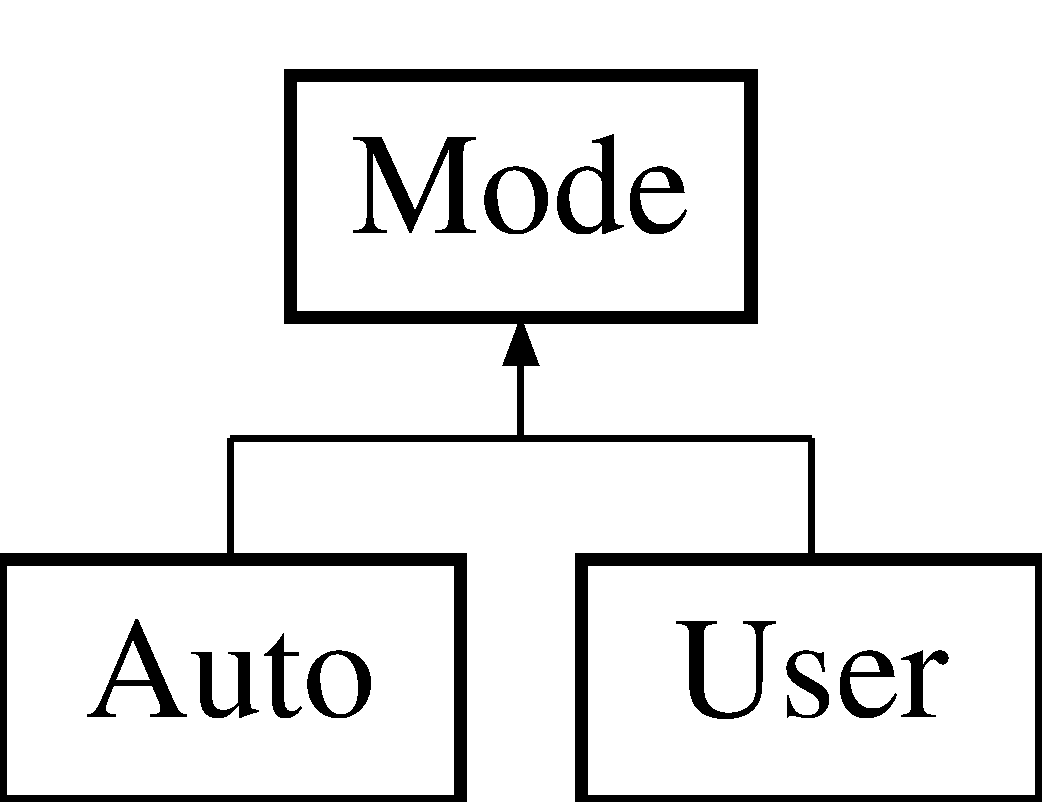
\includegraphics[height=2.000000cm]{struct_mode}
\end{center}
\end{figure}


\subsection{Detailed Description}
A struct encapsulating information about the match algorithm. 

The documentation for this struct was generated from the following file\-:\begin{DoxyCompactItemize}
\item 
D\-:/\-Seq\-An/\-Development/seqan-\/trunk/sandbox/my\-\_\-sandbox/apps/\-Seq\-D\-P\-T/\hyperlink{adapter_trimming_8h}{adapter\-Trimming.\-h}\end{DoxyCompactItemize}

\hypertarget{class_output_streams}{\section{Output\-Streams Class Reference}
\label{class_output_streams}\index{Output\-Streams@{Output\-Streams}}
}


Class that dynamically manages output streams that write out sets of sequences.  


\subsection*{Public Member Functions}
\begin{DoxyCompactItemize}
\item 
\hypertarget{class_output_streams_a224ac9f0321f3552b6874554e63683d7}{\hyperlink{class_output_streams_a224ac9f0321f3552b6874554e63683d7}{Output\-Streams} (seqan\-::\-Char\-String base, seqan\-::\-Seq\-I\-O\-File\-Format\-\_\-\-::\-Type format, bool compress)}\label{class_output_streams_a224ac9f0321f3552b6874554e63683d7}

\begin{DoxyCompactList}\small\item\em Constructor for the \hyperlink{class_output_streams}{Output\-Streams} object. Prepares the file extension which will be used for all streams created by this object and saves a base directory path. \end{DoxyCompactList}\item 
{\footnotesize template$<$typename T\-Key , typename T\-Map $>$ }\\bool \hyperlink{class_output_streams_a14babf33ab80c1dd5d158f2ddd9d5625}{exists} (T\-Key \&key, T\-Map \&map)
\begin{DoxyCompactList}\small\item\em Checks whether a key exists in a std\-::map. \end{DoxyCompactList}\item 
void \hyperlink{class_output_streams_a57fe721eed419cf693ad16ac2d065783}{add\-Stream} (seqan\-::\-Char\-String file\-Name, int id)
\begin{DoxyCompactList}\small\item\em Add a new output streams to the collection of streams. \end{DoxyCompactList}\item 
void \hyperlink{class_output_streams_ae724b4ed3aebd3ddd9d4426cdc6c856b}{add\-Streams} (seqan\-::\-Char\-String file\-Name1, seqan\-::\-Char\-String file\-Name2, int id)
\begin{DoxyCompactList}\small\item\em Add a new output streams to the collection of streams. \end{DoxyCompactList}\item 
{\footnotesize template$<$typename T\-Map , typename T\-Names $>$ }\\void \hyperlink{class_output_streams_aa807680b5625932c7cdd65c25023aaa3}{update\-Streams} (T\-Map \&map, T\-Names \&names, bool pair)
\begin{DoxyCompactList}\small\item\em This method takes a vector of numbers and checks if these numbers are already associated with a stream. If not, a new stream is added and the opened file is named according to the list of names. One or two files are created. \end{DoxyCompactList}\item 
{\footnotesize template$<$typename T\-Ids , typename T\-Seqs , typename T\-Map , typename T\-Names $>$ }\\void \hyperlink{class_output_streams_afcbc59e33ac5ea2487bd8db8dd3250c3}{write\-Seqs} (T\-Ids \&ids, T\-Seqs \&seqs, T\-Map \&map, T\-Names \&names)
\begin{DoxyCompactList}\small\item\em Writes the sets of ids and sequences to their corresponding files. \end{DoxyCompactList}\item 
{\footnotesize template$<$typename T\-Ids , typename T\-Seqs , typename T\-Map , typename T\-Names $>$ }\\void \hyperlink{class_output_streams_a4e2742f8208c6b37d6d5177e500ddac3}{write\-Seqs} (T\-Ids \&ids1, T\-Seqs \&seqs1, T\-Ids \&ids2, T\-Seqs \&seqs2, T\-Map \&map, T\-Names \&names)
\begin{DoxyCompactList}\small\item\em Writes the sets of ids and sequences to their corresponding files. Overload for writing paired-\/end sequence sets. \end{DoxyCompactList}\item 
\hypertarget{class_output_streams_a067d0c279e6148f9c46299b25616887e}{\hyperlink{class_output_streams_a067d0c279e6148f9c46299b25616887e}{$\sim$\-Output\-Streams} ()}\label{class_output_streams_a067d0c279e6148f9c46299b25616887e}

\begin{DoxyCompactList}\small\item\em Destructor of the object holding the output streams. Needed to destroy the streams properly after they have been created with new. \end{DoxyCompactList}\end{DoxyCompactItemize}


\subsection{Detailed Description}
Class that dynamically manages output streams that write out sets of sequences. 

\subsection{Member Function Documentation}
\hypertarget{class_output_streams_a57fe721eed419cf693ad16ac2d065783}{\index{Output\-Streams@{Output\-Streams}!add\-Stream@{add\-Stream}}
\index{add\-Stream@{add\-Stream}!OutputStreams@{Output\-Streams}}
\subsubsection[{add\-Stream}]{\setlength{\rightskip}{0pt plus 5cm}void Output\-Streams\-::add\-Stream (
\begin{DoxyParamCaption}
\item[{seqan\-::\-Char\-String}]{file\-Name, }
\item[{int}]{id}
\end{DoxyParamCaption}
)\hspace{0.3cm}{\ttfamily [inline]}}}\label{class_output_streams_a57fe721eed419cf693ad16ac2d065783}


Add a new output streams to the collection of streams. 


\begin{DoxyParams}{Parameters}
{\em file\-Name} & The name of the first file that will be created. \\
\hline
{\em id} & The associated id that will be used to identify the stream. \\
\hline
\end{DoxyParams}
\hypertarget{class_output_streams_ae724b4ed3aebd3ddd9d4426cdc6c856b}{\index{Output\-Streams@{Output\-Streams}!add\-Streams@{add\-Streams}}
\index{add\-Streams@{add\-Streams}!OutputStreams@{Output\-Streams}}
\subsubsection[{add\-Streams}]{\setlength{\rightskip}{0pt plus 5cm}void Output\-Streams\-::add\-Streams (
\begin{DoxyParamCaption}
\item[{seqan\-::\-Char\-String}]{file\-Name1, }
\item[{seqan\-::\-Char\-String}]{file\-Name2, }
\item[{int}]{id}
\end{DoxyParamCaption}
)\hspace{0.3cm}{\ttfamily [inline]}}}\label{class_output_streams_ae724b4ed3aebd3ddd9d4426cdc6c856b}


Add a new output streams to the collection of streams. 


\begin{DoxyParams}{Parameters}
{\em file\-Name1} & The name of the first file that will be created. \\
\hline
{\em file\-Name2} & The name of the second file that will be created. \\
\hline
{\em id} & The associated id that will be used to identify the pair of streams. \\
\hline
\end{DoxyParams}
\hypertarget{class_output_streams_a14babf33ab80c1dd5d158f2ddd9d5625}{\index{Output\-Streams@{Output\-Streams}!exists@{exists}}
\index{exists@{exists}!OutputStreams@{Output\-Streams}}
\subsubsection[{exists}]{\setlength{\rightskip}{0pt plus 5cm}template$<$typename T\-Key , typename T\-Map $>$ bool Output\-Streams\-::exists (
\begin{DoxyParamCaption}
\item[{T\-Key \&}]{key, }
\item[{T\-Map \&}]{map}
\end{DoxyParamCaption}
)\hspace{0.3cm}{\ttfamily [inline]}}}\label{class_output_streams_a14babf33ab80c1dd5d158f2ddd9d5625}


Checks whether a key exists in a std\-::map. 

\begin{DoxyReturn}{Returns}
True if the key exists, false otherwise. 
\end{DoxyReturn}
\hypertarget{class_output_streams_aa807680b5625932c7cdd65c25023aaa3}{\index{Output\-Streams@{Output\-Streams}!update\-Streams@{update\-Streams}}
\index{update\-Streams@{update\-Streams}!OutputStreams@{Output\-Streams}}
\subsubsection[{update\-Streams}]{\setlength{\rightskip}{0pt plus 5cm}template$<$typename T\-Map , typename T\-Names $>$ void Output\-Streams\-::update\-Streams (
\begin{DoxyParamCaption}
\item[{T\-Map \&}]{map, }
\item[{T\-Names \&}]{names, }
\item[{bool}]{pair}
\end{DoxyParamCaption}
)\hspace{0.3cm}{\ttfamily [inline]}}}\label{class_output_streams_aa807680b5625932c7cdd65c25023aaa3}


This method takes a vector of numbers and checks if these numbers are already associated with a stream. If not, a new stream is added and the opened file is named according to the list of names. One or two files are created. 


\begin{DoxyParams}{Parameters}
{\em map} & The list of I\-Ds for which the existence of a file should be checked. \\
\hline
{\em names} & The list of names to be used when creating new files. \\
\hline
{\em pair} & Indicates whether one or two (a pair of files) should be created. \\
\hline
\end{DoxyParams}
\hypertarget{class_output_streams_afcbc59e33ac5ea2487bd8db8dd3250c3}{\index{Output\-Streams@{Output\-Streams}!write\-Seqs@{write\-Seqs}}
\index{write\-Seqs@{write\-Seqs}!OutputStreams@{Output\-Streams}}
\subsubsection[{write\-Seqs}]{\setlength{\rightskip}{0pt plus 5cm}template$<$typename T\-Ids , typename T\-Seqs , typename T\-Map , typename T\-Names $>$ void Output\-Streams\-::write\-Seqs (
\begin{DoxyParamCaption}
\item[{T\-Ids \&}]{ids, }
\item[{T\-Seqs \&}]{seqs, }
\item[{T\-Map \&}]{map, }
\item[{T\-Names \&}]{names}
\end{DoxyParamCaption}
)\hspace{0.3cm}{\ttfamily [inline]}}}\label{class_output_streams_afcbc59e33ac5ea2487bd8db8dd3250c3}


Writes the sets of ids and sequences to their corresponding files. 


\begin{DoxyParams}{Parameters}
{\em ids} & A list of sets of sequence I\-Ds. (As returned by read\-Record etc.) \\
\hline
{\em seqs} & A list of sets of sequences. \\
\hline
{\em map} & A mapping of the sets of sequences to their corresponding output streams. \\
\hline
{\em names} & Names to be used when creating new streams. \\
\hline
\end{DoxyParams}
\hypertarget{class_output_streams_a4e2742f8208c6b37d6d5177e500ddac3}{\index{Output\-Streams@{Output\-Streams}!write\-Seqs@{write\-Seqs}}
\index{write\-Seqs@{write\-Seqs}!OutputStreams@{Output\-Streams}}
\subsubsection[{write\-Seqs}]{\setlength{\rightskip}{0pt plus 5cm}template$<$typename T\-Ids , typename T\-Seqs , typename T\-Map , typename T\-Names $>$ void Output\-Streams\-::write\-Seqs (
\begin{DoxyParamCaption}
\item[{T\-Ids \&}]{ids1, }
\item[{T\-Seqs \&}]{seqs1, }
\item[{T\-Ids \&}]{ids2, }
\item[{T\-Seqs \&}]{seqs2, }
\item[{T\-Map \&}]{map, }
\item[{T\-Names \&}]{names}
\end{DoxyParamCaption}
)\hspace{0.3cm}{\ttfamily [inline]}}}\label{class_output_streams_a4e2742f8208c6b37d6d5177e500ddac3}


Writes the sets of ids and sequences to their corresponding files. Overload for writing paired-\/end sequence sets. 


\begin{DoxyParams}{Parameters}
{\em ids1} & A list of sets of forward sequence I\-Ds. (As returned by read\-Record etc.) \\
\hline
{\em seqs1} & A list of sets of forward sequences. \\
\hline
{\em ids2} & A list of sets of backward sequence I\-Ds. (As returned by read\-Record etc.) \\
\hline
{\em seqs2} & A list of sets of backward sequences. \\
\hline
{\em map} & A mapping of the sets of sequences to their corresponding output streams. \\
\hline
{\em names} & Names to be used when creating new streams. \\
\hline
\end{DoxyParams}


The documentation for this class was generated from the following file\-:\begin{DoxyCompactItemize}
\item 
D\-:/\-Seq\-An/\-Development/seqan-\/trunk/sandbox/my\-\_\-sandbox/apps/\-Seq\-D\-P\-T/Seq\-D\-P\-T.\-cpp\end{DoxyCompactItemize}

\hypertarget{struct_program_params}{\section{Program\-Params Struct Reference}
\label{struct_program_params}\index{Program\-Params@{Program\-Params}}
}


Struct that hold program parameters that might need to be available at multiple places in the program.  


\subsection*{Public Attributes}
\begin{DoxyCompactItemize}
\item 
\hypertarget{struct_program_params_a70461e1706b9ca1639b271454d602852}{int {\bfseries file\-Count}}\label{struct_program_params_a70461e1706b9ca1639b271454d602852}

\item 
\hypertarget{struct_program_params_a8deb8c9b0c8e1d6e4edde11298f88954}{int {\bfseries read\-Count}}\label{struct_program_params_a8deb8c9b0c8e1d6e4edde11298f88954}

\item 
\hypertarget{struct_program_params_a108ec56ae620ce7e0ca40fa050f6a93a}{double {\bfseries process\-Time}}\label{struct_program_params_a108ec56ae620ce7e0ca40fa050f6a93a}

\item 
\hypertarget{struct_program_params_a89fcbdab4dbb81042ac81681c490f01c}{double {\bfseries io\-Time}}\label{struct_program_params_a89fcbdab4dbb81042ac81681c490f01c}

\item 
\hypertarget{struct_program_params_a81969e289b361114586bbd26c03d99b6}{seqan\-::\-Sequence\-Stream {\bfseries file\-Stream1}}\label{struct_program_params_a81969e289b361114586bbd26c03d99b6}

\item 
\hypertarget{struct_program_params_a7b47e0313a409c5b932aa8c1074118ca}{seqan\-::\-Sequence\-Stream {\bfseries file\-Stream2}}\label{struct_program_params_a7b47e0313a409c5b932aa8c1074118ca}

\end{DoxyCompactItemize}


\subsection{Detailed Description}
Struct that hold program parameters that might need to be available at multiple places in the program. 

The documentation for this struct was generated from the following file\-:\begin{DoxyCompactItemize}
\item 
D\-:/\-Seq\-An/\-Development/seqan-\/trunk/sandbox/my\-\_\-sandbox/apps/\-Seq\-D\-P\-T/Seq\-D\-P\-T.\-cpp\end{DoxyCompactItemize}

\hypertarget{struct_quality_trimming_params}{\section{Quality\-Trimming\-Params Struct Reference}
\label{struct_quality_trimming_params}\index{Quality\-Trimming\-Params@{Quality\-Trimming\-Params}}
}


Struct holding all quality trimming parameters.  


\subsection*{Public Attributes}
\begin{DoxyCompactItemize}
\item 
Trimming\-Mode \hyperlink{struct_quality_trimming_params_a048e76b525de1500f55f39e9e572ab80}{trim\-\_\-mode}
\item 
int \hyperlink{struct_quality_trimming_params_a3b2b268123a0054eda2f603e7be590dc}{cutoff}
\item 
int \hyperlink{struct_quality_trimming_params_a754750a0a278d17d82a02dedfbf185ba}{min\-\_\-length}
\item 
bool \hyperlink{struct_quality_trimming_params_a1b2db8d78cae5e3db9d8fc903e042310}{run}
\item 
\hyperlink{struct_quality_trimming_stats}{Quality\-Trimming\-Stats} \hyperlink{struct_quality_trimming_params_a5f07878380511531b124c6f94a611b91}{stats}
\end{DoxyCompactItemize}


\subsection{Detailed Description}
Struct holding all quality trimming parameters. 

Struct holding the parameters needed for quality trimming. 

\subsection{Member Data Documentation}
\hypertarget{struct_quality_trimming_params_a3b2b268123a0054eda2f603e7be590dc}{\index{Quality\-Trimming\-Params@{Quality\-Trimming\-Params}!cutoff@{cutoff}}
\index{cutoff@{cutoff}!QualityTrimmingParams@{Quality\-Trimming\-Params}}
\subsubsection[{cutoff}]{\setlength{\rightskip}{0pt plus 5cm}int Quality\-Trimming\-Params\-::cutoff}}\label{struct_quality_trimming_params_a3b2b268123a0054eda2f603e7be590dc}
Holds the cutoff score. \hypertarget{struct_quality_trimming_params_a754750a0a278d17d82a02dedfbf185ba}{\index{Quality\-Trimming\-Params@{Quality\-Trimming\-Params}!min\-\_\-length@{min\-\_\-length}}
\index{min\-\_\-length@{min\-\_\-length}!QualityTrimmingParams@{Quality\-Trimming\-Params}}
\subsubsection[{min\-\_\-length}]{\setlength{\rightskip}{0pt plus 5cm}int Quality\-Trimming\-Params\-::min\-\_\-length}}\label{struct_quality_trimming_params_a754750a0a278d17d82a02dedfbf185ba}
Holds the minam length of a sequnce after trimming. \hypertarget{struct_quality_trimming_params_a1b2db8d78cae5e3db9d8fc903e042310}{\index{Quality\-Trimming\-Params@{Quality\-Trimming\-Params}!run@{run}}
\index{run@{run}!QualityTrimmingParams@{Quality\-Trimming\-Params}}
\subsubsection[{run}]{\setlength{\rightskip}{0pt plus 5cm}bool Quality\-Trimming\-Params\-::run}}\label{struct_quality_trimming_params_a1b2db8d78cae5e3db9d8fc903e042310}
T\-R\-U\-E if the quality trimming shall run. \hypertarget{struct_quality_trimming_params_a5f07878380511531b124c6f94a611b91}{\index{Quality\-Trimming\-Params@{Quality\-Trimming\-Params}!stats@{stats}}
\index{stats@{stats}!QualityTrimmingParams@{Quality\-Trimming\-Params}}
\subsubsection[{stats}]{\setlength{\rightskip}{0pt plus 5cm}{\bf Quality\-Trimming\-Stats} Quality\-Trimming\-Params\-::stats}}\label{struct_quality_trimming_params_a5f07878380511531b124c6f94a611b91}
Holds interesting numbers about quality trimming. \hypertarget{struct_quality_trimming_params_a048e76b525de1500f55f39e9e572ab80}{\index{Quality\-Trimming\-Params@{Quality\-Trimming\-Params}!trim\-\_\-mode@{trim\-\_\-mode}}
\index{trim\-\_\-mode@{trim\-\_\-mode}!QualityTrimmingParams@{Quality\-Trimming\-Params}}
\subsubsection[{trim\-\_\-mode}]{\setlength{\rightskip}{0pt plus 5cm}Trimming\-Mode Quality\-Trimming\-Params\-::trim\-\_\-mode}}\label{struct_quality_trimming_params_a048e76b525de1500f55f39e9e572ab80}
Holds the \-::\-Trimming\-Algorithm-\/object which determines which algrotihm shall be used. 

The documentation for this struct was generated from the following file\-:\begin{DoxyCompactItemize}
\item 
D\-:/\-Seq\-An/\-Development/seqan-\/trunk/sandbox/my\-\_\-sandbox/apps/\-Seq\-D\-P\-T/Seq\-D\-P\-T.\-cpp\end{DoxyCompactItemize}

\hypertarget{struct_quality_trimming_stats}{\section{Quality\-Trimming\-Stats Struct Reference}
\label{struct_quality_trimming_stats}\index{Quality\-Trimming\-Stats@{Quality\-Trimming\-Stats}}
}
\subsection*{Public Member Functions}
\begin{DoxyCompactItemize}
\item 
\hypertarget{struct_quality_trimming_stats_afbf166ddb242c870cdb271c8bfa81bd4}{void {\bfseries clear} ()}\label{struct_quality_trimming_stats_afbf166ddb242c870cdb271c8bfa81bd4}

\end{DoxyCompactItemize}
\subsection*{Public Attributes}
\begin{DoxyCompactItemize}
\item 
\hypertarget{struct_quality_trimming_stats_a2a3f9b43f0112d825bb1043d64255428}{unsigned {\bfseries dropped\-\_\-1}}\label{struct_quality_trimming_stats_a2a3f9b43f0112d825bb1043d64255428}

\item 
\hypertarget{struct_quality_trimming_stats_ab5c4b6046520e4279cd2000fef5983ef}{unsigned {\bfseries dropped\-\_\-2}}\label{struct_quality_trimming_stats_ab5c4b6046520e4279cd2000fef5983ef}

\end{DoxyCompactItemize}


The documentation for this struct was generated from the following file\-:\begin{DoxyCompactItemize}
\item 
D\-:/\-Seq\-An/\-Development/seqan-\/trunk/sandbox/my\-\_\-sandbox/apps/\-Seq\-D\-P\-T/\hyperlink{read_trimming_8h}{read\-Trimming.\-h}\end{DoxyCompactItemize}

\hypertarget{structseqan_1_1_scoring_matrix_data___3_01int_00_01_dna5_00_01_adapter_scoring_matrix_01_4}{\section{seqan\-:\-:Scoring\-Matrix\-Data\-\_\-$<$ int, Dna5, Adapter\-Scoring\-Matrix $>$ Struct Template Reference}
\label{structseqan_1_1_scoring_matrix_data___3_01int_00_01_dna5_00_01_adapter_scoring_matrix_01_4}\index{seqan\-::\-Scoring\-Matrix\-Data\-\_\-$<$ int, Dna5, Adapter\-Scoring\-Matrix $>$@{seqan\-::\-Scoring\-Matrix\-Data\-\_\-$<$ int, Dna5, Adapter\-Scoring\-Matrix $>$}}
}


Struct containing data for the \hyperlink{structseqan_1_1_adapter_scoring_matrix}{seqan\-::\-Adapter\-Scoring\-Matrix} custom scoring matrix. Matches score 1, mismatches -\/1 and matches against N with 0.  




{\ttfamily \#include $<$adapter\-Trimming.\-h$>$}

\subsection*{Public Types}
\begin{DoxyCompactItemize}
\item 
enum \{ {\bfseries V\-A\-L\-U\-E\-\_\-\-S\-I\-Z\-E} = Value\-Size$<$Dna5$>$\-:\-:V\-A\-L\-U\-E, 
{\bfseries T\-A\-B\-\_\-\-S\-I\-Z\-E} = V\-A\-L\-U\-E\-\_\-\-S\-I\-Z\-E $\ast$ V\-A\-L\-U\-E\-\_\-\-S\-I\-Z\-E
 \}
\end{DoxyCompactItemize}
\subsection*{Static Public Member Functions}
\begin{DoxyCompactItemize}
\item 
\hypertarget{structseqan_1_1_scoring_matrix_data___3_01int_00_01_dna5_00_01_adapter_scoring_matrix_01_4_a77db480cd1d3f5e2c98b32af0c38716c}{static int const $\ast$ {\bfseries get\-Data} ()}\label{structseqan_1_1_scoring_matrix_data___3_01int_00_01_dna5_00_01_adapter_scoring_matrix_01_4_a77db480cd1d3f5e2c98b32af0c38716c}

\end{DoxyCompactItemize}


\subsection{Detailed Description}
\subsubsection*{template$<$$>$struct seqan\-::\-Scoring\-Matrix\-Data\-\_\-$<$ int, Dna5, Adapter\-Scoring\-Matrix $>$}

Struct containing data for the \hyperlink{structseqan_1_1_adapter_scoring_matrix}{seqan\-::\-Adapter\-Scoring\-Matrix} custom scoring matrix. Matches score 1, mismatches -\/1 and matches against N with 0. 

The documentation for this struct was generated from the following file\-:\begin{DoxyCompactItemize}
\item 
D\-:/\-Seq\-An/\-Development/seqan-\/trunk/sandbox/my\-\_\-sandbox/apps/\-Seq\-D\-P\-T/\hyperlink{adapter_trimming_8h}{adapter\-Trimming.\-h}\end{DoxyCompactItemize}

\hypertarget{struct_s_t_r_i_n_g___r_e_v_e_r_s_e___c_o_m_p_l_e_m_e_n_t}{\section{S\-T\-R\-I\-N\-G\-\_\-\-R\-E\-V\-E\-R\-S\-E\-\_\-\-C\-O\-M\-P\-L\-E\-M\-E\-N\-T$<$ T\-Value $>$ Struct Template Reference}
\label{struct_s_t_r_i_n_g___r_e_v_e_r_s_e___c_o_m_p_l_e_m_e_n_t}\index{S\-T\-R\-I\-N\-G\-\_\-\-R\-E\-V\-E\-R\-S\-E\-\_\-\-C\-O\-M\-P\-L\-E\-M\-E\-N\-T$<$ T\-Value $>$@{S\-T\-R\-I\-N\-G\-\_\-\-R\-E\-V\-E\-R\-S\-E\-\_\-\-C\-O\-M\-P\-L\-E\-M\-E\-N\-T$<$ T\-Value $>$}}
}


A metafunction which constructs a Modified\-String type for an Alphabet.  




{\ttfamily \#include $<$adapter\-Trimming.\-h$>$}

\subsection*{Public Types}
\begin{DoxyCompactItemize}
\item 
\hypertarget{struct_s_t_r_i_n_g___r_e_v_e_r_s_e___c_o_m_p_l_e_m_e_n_t_a6bd7f83c07f52c09bc4e5304fb416fb7}{typedef Modified\-String\\*
$<$ Modified\-String$<$ String\\*
$<$ T\-Value $>$, Mod\-View\\*
$<$ Functor\-Complement$<$ T\-Value $>$\\*
 $>$ $>$, Mod\-Reverse $>$ {\bfseries Type}}\label{struct_s_t_r_i_n_g___r_e_v_e_r_s_e___c_o_m_p_l_e_m_e_n_t_a6bd7f83c07f52c09bc4e5304fb416fb7}

\end{DoxyCompactItemize}


\subsection{Detailed Description}
\subsubsection*{template$<$class T\-Value$>$struct S\-T\-R\-I\-N\-G\-\_\-\-R\-E\-V\-E\-R\-S\-E\-\_\-\-C\-O\-M\-P\-L\-E\-M\-E\-N\-T$<$ T\-Value $>$}

A metafunction which constructs a Modified\-String type for an Alphabet. 

The documentation for this struct was generated from the following file\-:\begin{DoxyCompactItemize}
\item 
D\-:/\-Seq\-An/\-Development/seqan-\/trunk/sandbox/my\-\_\-sandbox/apps/\-Seq\-D\-P\-T/\hyperlink{adapter_trimming_8h}{adapter\-Trimming.\-h}\end{DoxyCompactItemize}

\hypertarget{struct_tail}{\section{Tail Struct Reference}
\label{struct_tail}\index{Tail@{Tail}}
}


The tagging structure for the \hyperlink{struct_tail}{Tail} trimming algorithm.  




{\ttfamily \#include $<$read\-Trimming.\-h$>$}



\subsection{Detailed Description}
The tagging structure for the \hyperlink{struct_tail}{Tail} trimming algorithm. 

The documentation for this struct was generated from the following file\-:\begin{DoxyCompactItemize}
\item 
D\-:/\-Seq\-An/\-Development/seqan-\/trunk/sandbox/my\-\_\-sandbox/apps/\-Seq\-D\-P\-T/\hyperlink{read_trimming_8h}{read\-Trimming.\-h}\end{DoxyCompactItemize}

\hypertarget{struct_user}{\section{User Struct Reference}
\label{struct_user}\index{User@{User}}
}


Tagging struct representing the the match algorithm working with values supplied by the user. Saves those values as members.  




{\ttfamily \#include $<$adapter\-Trimming.\-h$>$}

Inheritance diagram for User\-:\begin{figure}[H]
\begin{center}
\leavevmode
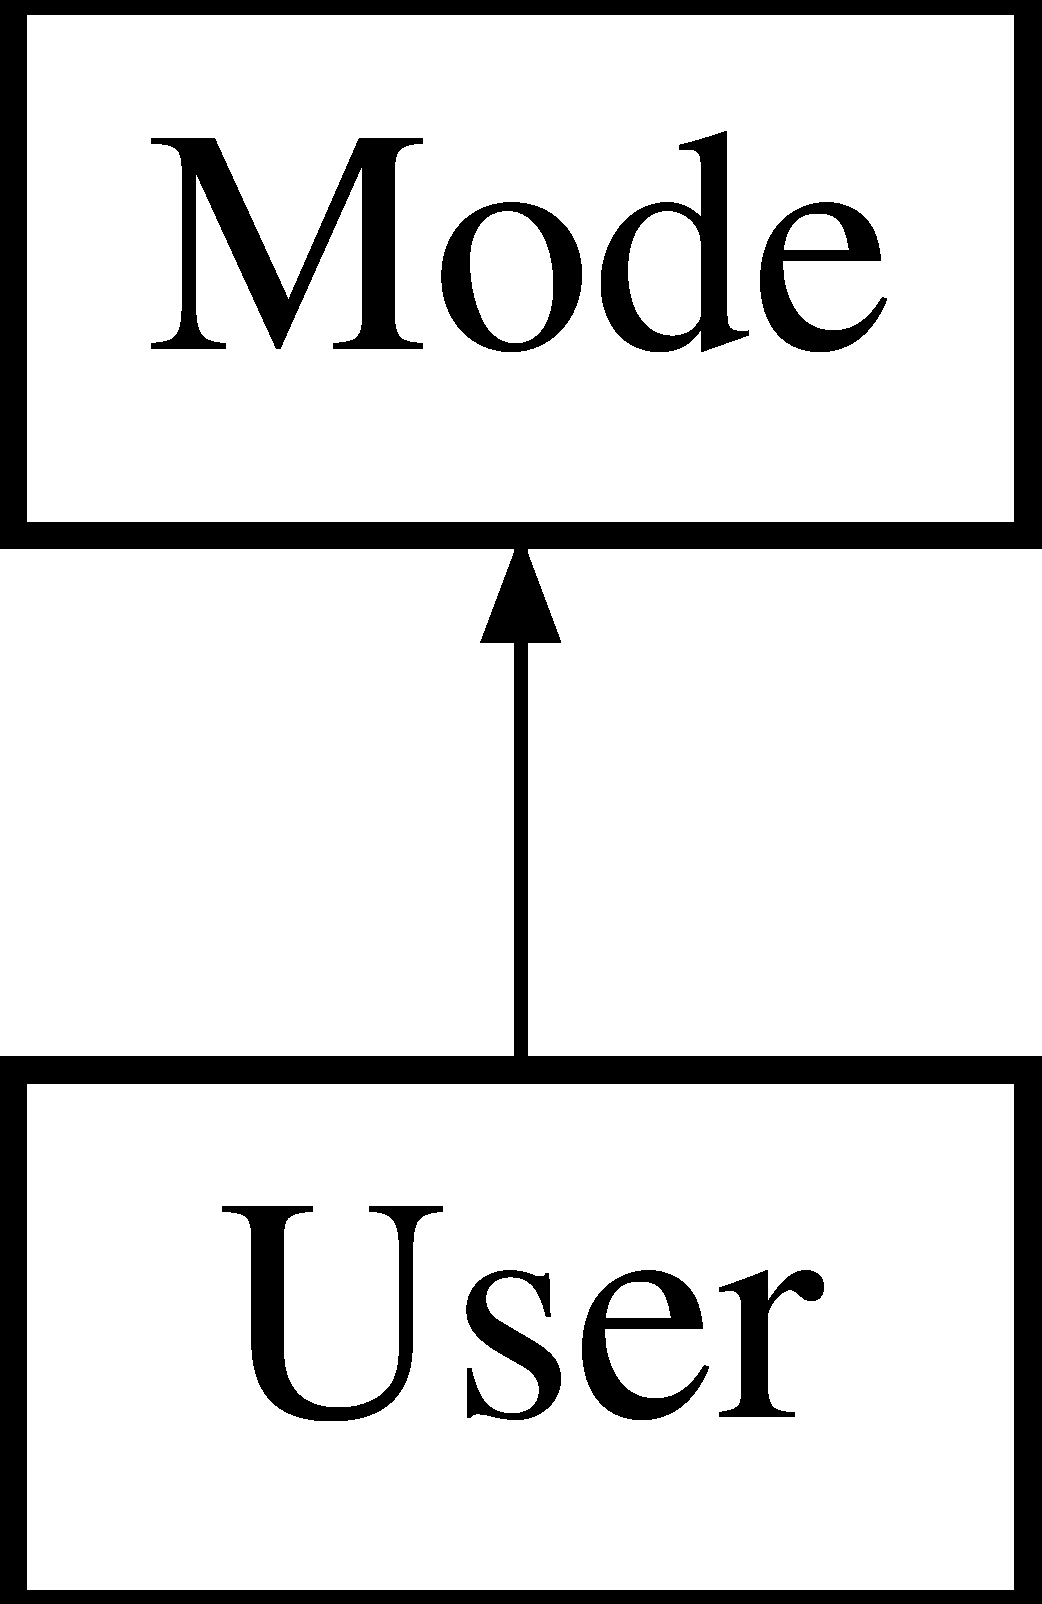
\includegraphics[height=2.000000cm]{struct_user}
\end{center}
\end{figure}
\subsection*{Public Member Functions}
\begin{DoxyCompactItemize}
\item 
\hypertarget{struct_user_a522ee72180516ce491c9e495530a6f34}{{\bfseries User} (int m, int e)}\label{struct_user_a522ee72180516ce491c9e495530a6f34}

\end{DoxyCompactItemize}
\subsection*{Public Attributes}
\begin{DoxyCompactItemize}
\item 
int \hyperlink{struct_user_ae94113fb04b477ed27af1e0fe9e7822e}{min\-\_\-length}
\item 
int \hyperlink{struct_user_a8622c0446a3a49852b69c5d558a62d7c}{errors}
\end{DoxyCompactItemize}


\subsection{Detailed Description}
Tagging struct representing the the match algorithm working with values supplied by the user. Saves those values as members. 

\subsection{Member Data Documentation}
\hypertarget{struct_user_a8622c0446a3a49852b69c5d558a62d7c}{\index{User@{User}!errors@{errors}}
\index{errors@{errors}!User@{User}}
\subsubsection[{errors}]{\setlength{\rightskip}{0pt plus 5cm}int User\-::errors}}\label{struct_user_a8622c0446a3a49852b69c5d558a62d7c}
The maximum number of errors we allow. \hypertarget{struct_user_ae94113fb04b477ed27af1e0fe9e7822e}{\index{User@{User}!min\-\_\-length@{min\-\_\-length}}
\index{min\-\_\-length@{min\-\_\-length}!User@{User}}
\subsubsection[{min\-\_\-length}]{\setlength{\rightskip}{0pt plus 5cm}int User\-::min\-\_\-length}}\label{struct_user_ae94113fb04b477ed27af1e0fe9e7822e}
The minimum length of the overlap. 

The documentation for this struct was generated from the following file\-:\begin{DoxyCompactItemize}
\item 
D\-:/\-Seq\-An/\-Development/seqan-\/trunk/sandbox/my\-\_\-sandbox/apps/\-Seq\-D\-P\-T/\hyperlink{adapter_trimming_8h}{adapter\-Trimming.\-h}\end{DoxyCompactItemize}

\chapter{File Documentation}
\hypertarget{adapter_trimming_8h}{\section{D\-:/\-Seq\-An/\-Development/seqan-\/trunk/sandbox/my\-\_\-sandbox/apps/\-Seq\-D\-P\-T/adapter\-Trimming.h File Reference}
\label{adapter_trimming_8h}\index{D\-:/\-Seq\-An/\-Development/seqan-\/trunk/sandbox/my\-\_\-sandbox/apps/\-Seq\-D\-P\-T/adapter\-Trimming.\-h@{D\-:/\-Seq\-An/\-Development/seqan-\/trunk/sandbox/my\-\_\-sandbox/apps/\-Seq\-D\-P\-T/adapter\-Trimming.\-h}}
}


Contains the functions for adapter trimming.  


{\ttfamily \#include $<$seqan/align.\-h$>$}\\*
{\ttfamily \#include $<$seqan/find.\-h$>$}\\*
\subsection*{Classes}
\begin{DoxyCompactItemize}
\item 
struct \hyperlink{structseqan_1_1_adapter_scoring_matrix}{seqan\-::\-Adapter\-Scoring\-Matrix}
\begin{DoxyCompactList}\small\item\em Struct used to define a new custom scoring matrix. \end{DoxyCompactList}\item 
struct \hyperlink{structseqan_1_1_scoring_matrix_data___3_01int_00_01_dna5_00_01_adapter_scoring_matrix_01_4}{seqan\-::\-Scoring\-Matrix\-Data\-\_\-$<$ int, Dna5, Adapter\-Scoring\-Matrix $>$}
\begin{DoxyCompactList}\small\item\em Struct containing data for the \hyperlink{structseqan_1_1_adapter_scoring_matrix}{seqan\-::\-Adapter\-Scoring\-Matrix} custom scoring matrix. Matches score 1, mismatches -\/1 and matches against N with 0. \end{DoxyCompactList}\item 
struct \hyperlink{struct_mode}{Mode}
\begin{DoxyCompactList}\small\item\em A struct encapsulating information about the match algorithm. \end{DoxyCompactList}\item 
struct \hyperlink{struct_auto}{Auto}
\begin{DoxyCompactList}\small\item\em Tagging struct for the automatic match algorithm. \end{DoxyCompactList}\item 
struct \hyperlink{struct_user}{User}
\begin{DoxyCompactList}\small\item\em Tagging struct representing the the match algorithm working with values supplied by the user. Saves those values as members. \end{DoxyCompactList}\item 
struct \hyperlink{struct_adapter_trimming_stats}{Adapter\-Trimming\-Stats}
\begin{DoxyCompactList}\small\item\em Struct holding information about certain adapter trimming statistics. \end{DoxyCompactList}\item 
struct \hyperlink{struct_s_t_r_i_n_g___r_e_v_e_r_s_e___c_o_m_p_l_e_m_e_n_t}{S\-T\-R\-I\-N\-G\-\_\-\-R\-E\-V\-E\-R\-S\-E\-\_\-\-C\-O\-M\-P\-L\-E\-M\-E\-N\-T$<$ T\-Value $>$}
\begin{DoxyCompactList}\small\item\em A metafunction which constructs a Modified\-String type for an Alphabet. \end{DoxyCompactList}\end{DoxyCompactItemize}
\subsection*{Typedefs}
\begin{DoxyCompactItemize}
\item 
\hypertarget{adapter_trimming_8h_ab719b1a56b7f138316a70a055c8ae54e}{typedef Score$<$ int, \\*
Score\-Matrix$<$ Dna5, \\*
\hyperlink{structseqan_1_1_adapter_scoring_matrix}{Adapter\-Scoring\-Matrix} $>$ $>$ {\bfseries T\-Score}}\label{adapter_trimming_8h_ab719b1a56b7f138316a70a055c8ae54e}

\end{DoxyCompactItemize}
\subsection*{Functions}
\begin{DoxyCompactItemize}
\item 
{\footnotesize template$<$typename T\-Seq1 , typename T\-Seq2 , bool T\-Top, bool T\-Left, bool T\-Right, bool T\-Bottom$>$ }\\seqan\-::\-Pair$<$ unsigned, \\*
seqan\-::\-Align$<$ T\-Seq1 $>$ $>$ \hyperlink{adapter_trimming_8h_a690b4222b093c2260ab0522bff30049f}{align\-Pair} (T\-Seq1 \&seq1, T\-Seq2 \&seq2, const seqan\-::\-Align\-Config$<$ T\-Top, T\-Left, T\-Right, T\-Bottom $>$ \&config, bool band=false)
\begin{DoxyCompactList}\small\item\em Align two sequences, returning the score and align object of the alignment. \end{DoxyCompactList}\item 
{\footnotesize template$<$typename T\-Row $>$ }\\unsigned \hyperlink{adapter_trimming_8h_a3bc646d4dc99acf0ae165cf082e217cb}{count\-Total\-Gaps} (T\-Row \&row)
\begin{DoxyCompactList}\small\item\em Returns the total number of gaps in a row object. \end{DoxyCompactList}\item 
{\footnotesize template$<$typename T\-Align $>$ }\\unsigned \hyperlink{adapter_trimming_8h_af28bd342d3520fd7fe6e298e0271e288}{get\-Overlap} (T\-Align \&align)
\begin{DoxyCompactList}\small\item\em Determines the overlap between two (free-\/shift) aligned gapless sequences. \end{DoxyCompactList}\item 
{\footnotesize template$<$typename T\-Align $>$ }\\unsigned \hyperlink{adapter_trimming_8h_a8427805bc99660a9476176b62061f45f}{get\-Insert\-Size} (T\-Align \&align)
\begin{DoxyCompactList}\small\item\em Given an alignment with two overlapping (forward and reverse) sequences, this function determines the actual size of the insert they cover. \end{DoxyCompactList}\item 
{\footnotesize template$<$typename T\-Seq $>$ }\\unsigned \hyperlink{adapter_trimming_8h_a502e2eb7a85e1f67dd637e94f1600524}{strip\-Pair} (T\-Seq \&seq1, T\-Seq \&seq2)
\begin{DoxyCompactList}\small\item\em Removes adapter contamination from paired-\/end reads. \end{DoxyCompactList}\item 
{\footnotesize template$<$typename T\-Seq $>$ }\\unsigned \hyperlink{adapter_trimming_8h_aeddd7c1ce0243088be7cde1b4cb5825c}{strip\-Pair} (T\-Seq \&seq1, T\-Seq \&adapter1, T\-Seq \&seq2, T\-Seq \&adapter2)
\begin{DoxyCompactList}\small\item\em Removes adapter contamination from paired-\/end reads with adapter information. \end{DoxyCompactList}\item 
{\footnotesize template$<$typename T\-Seq $>$ }\\unsigned \hyperlink{adapter_trimming_8h_a390ded6489d24d870c5b63d57b394ad9}{strip\-Pair\-Batch} (seqan\-::\-String\-Set$<$ T\-Seq $>$ \&set1, seqan\-::\-String\-Set$<$ T\-Seq $>$ \&set2, \hyperlink{struct_adapter_trimming_stats}{Adapter\-Trimming\-Stats} \&stats)
\begin{DoxyCompactList}\small\item\em Removes adapter contamination from paired-\/end reads. \end{DoxyCompactList}\item 
{\footnotesize template$<$typename T\-Seq , typename T\-Adapter $>$ }\\seqan\-::\-Pair$<$ unsigned, \\*
seqan\-::\-Align$<$ T\-Seq $>$ $>$ \hyperlink{adapter_trimming_8h_a5c6fd3864a1835e6d7120555021326ee}{align\-Adapter} (T\-Seq \&seq, T\-Adapter \&adapter)
\begin{DoxyCompactList}\small\item\em Aligns a sequence to an adapter. \end{DoxyCompactList}\item 
bool \hyperlink{adapter_trimming_8h_a8d41cfe5174b6faee428503c8fd0fa45}{is\-Match} (int overlap, int mismatches, const \hyperlink{struct_auto}{Auto} \&)
\begin{DoxyCompactList}\small\item\em Checks if a overlap of an alignment is accepted, based on mismatches and the length of the overlap. \end{DoxyCompactList}\item 
bool \hyperlink{adapter_trimming_8h_acd23c187993f2c93b6c9177d7df4563f}{is\-Match} (int overlap, int mismatches, const \hyperlink{struct_user}{User} \&user\-Options)
\begin{DoxyCompactList}\small\item\em Checks if a overlap of an alignment is accepted, based on mismatches and the length of the overlap. \end{DoxyCompactList}\item 
{\footnotesize template$<$typename T\-Seq , typename T\-Adapter , typename T\-Spec $>$ }\\unsigned \hyperlink{adapter_trimming_8h_a7f0ed5b254d423dabfb235c79355242d}{strip\-Adapter} (T\-Seq \&seq, T\-Adapter \&adapter, T\-Spec \&spec)
\begin{DoxyCompactList}\small\item\em Remove adapter sequence from a sequence. \end{DoxyCompactList}\item 
{\footnotesize template$<$typename T\-Seq , typename T\-Adapter , typename T\-Spec $>$ }\\unsigned \hyperlink{adapter_trimming_8h_a3c85c17ed0ce3241d328d9b609d88789}{strip\-Adapter\-Batch} (seqan\-::\-String\-Set$<$ T\-Seq $>$ \&set, T\-Adapter \&adapter, T\-Spec const \&spec, \hyperlink{struct_adapter_trimming_stats}{Adapter\-Trimming\-Stats} \&stats, bool reverse=false)
\begin{DoxyCompactList}\small\item\em Remove adapter sequence from a set of sequences. \end{DoxyCompactList}\item 
{\footnotesize template$<$typename T\-Seq , typename T\-Spec $>$ }\\unsigned \hyperlink{adapter_trimming_8h_a388d9f7c52eada005728f2394f2bb7d2}{strip\-Reverse\-Adapter\-Batch} (seqan\-::\-String\-Set$<$ T\-Seq $>$ \&set, T\-Seq \&adapter, T\-Spec const \&spec, \hyperlink{struct_adapter_trimming_stats}{Adapter\-Trimming\-Stats} \&stats)
\begin{DoxyCompactList}\small\item\em Simple interface to align the reverse complement of an adapter to a batch of sequences. to a set of reads and remove significant matches. \end{DoxyCompactList}\end{DoxyCompactItemize}


\subsection{Detailed Description}
Contains the functions for adapter trimming. 

\subsection{Function Documentation}
\hypertarget{adapter_trimming_8h_a5c6fd3864a1835e6d7120555021326ee}{\index{adapter\-Trimming.\-h@{adapter\-Trimming.\-h}!align\-Adapter@{align\-Adapter}}
\index{align\-Adapter@{align\-Adapter}!adapterTrimming.h@{adapter\-Trimming.\-h}}
\subsubsection[{align\-Adapter}]{\setlength{\rightskip}{0pt plus 5cm}template$<$typename T\-Seq , typename T\-Adapter $>$ seqan\-::\-Pair$<$unsigned, seqan\-::\-Align$<$T\-Seq$>$ $>$ align\-Adapter (
\begin{DoxyParamCaption}
\item[{T\-Seq \&}]{seq, }
\item[{T\-Adapter \&}]{adapter}
\end{DoxyParamCaption}
)}}\label{adapter_trimming_8h_a5c6fd3864a1835e6d7120555021326ee}


Aligns a sequence to an adapter. 


\begin{DoxyParams}{Parameters}
{\em seq} & The sequence which adapter contamination shall be removed. \\
\hline
{\em adapter} & The adapter that might contaminate the sequence. \\
\hline
\end{DoxyParams}
\begin{DoxyReturn}{Returns}
A pair of unsigned ints containing the score of the alignment and the alignment object. 
\end{DoxyReturn}
\hypertarget{adapter_trimming_8h_a690b4222b093c2260ab0522bff30049f}{\index{adapter\-Trimming.\-h@{adapter\-Trimming.\-h}!align\-Pair@{align\-Pair}}
\index{align\-Pair@{align\-Pair}!adapterTrimming.h@{adapter\-Trimming.\-h}}
\subsubsection[{align\-Pair}]{\setlength{\rightskip}{0pt plus 5cm}template$<$typename T\-Seq1 , typename T\-Seq2 , bool T\-Top, bool T\-Left, bool T\-Right, bool T\-Bottom$>$ seqan\-::\-Pair$<$unsigned, seqan\-::\-Align$<$T\-Seq1$>$ $>$ align\-Pair (
\begin{DoxyParamCaption}
\item[{T\-Seq1 \&}]{seq1, }
\item[{T\-Seq2 \&}]{seq2, }
\item[{const seqan\-::\-Align\-Config$<$ T\-Top, T\-Left, T\-Right, T\-Bottom $>$ \&}]{config, }
\item[{bool}]{band = {\ttfamily false}}
\end{DoxyParamCaption}
)}}\label{adapter_trimming_8h_a690b4222b093c2260ab0522bff30049f}


Align two sequences, returning the score and align object of the alignment. 


\begin{DoxyParams}{Parameters}
{\em seq1} & The first sequence of the alignment. \\
\hline
{\em seq2} & The second sequence of the alignment. \\
\hline
{\em config} & The alignment configuration used by the Seqan's global\-Alignment method. \\
\hline
{\em band} & Whether the alignment's lower diagonal should be banded at -\/2. (Two diagonals below the main diagonal.) Useful to speed up computation for 5'-\/3' overlap alignments. \\
\hline
\end{DoxyParams}
\begin{DoxyRemark}{Remarks}
The main intended uses are Align\-Config$<$true, false, true, false$>$ with band = true and Align\-Config$<$true, true, true, true$>$ with band = false. 

We use a custom scoring scheme which scores 1 for match, -\/1 for mismatch, 0 for match with N. 
\end{DoxyRemark}
\begin{DoxyReturn}{Returns}
A pair containing the score of the alignment and the aling object. 
\end{DoxyReturn}
\hypertarget{adapter_trimming_8h_a3bc646d4dc99acf0ae165cf082e217cb}{\index{adapter\-Trimming.\-h@{adapter\-Trimming.\-h}!count\-Total\-Gaps@{count\-Total\-Gaps}}
\index{count\-Total\-Gaps@{count\-Total\-Gaps}!adapterTrimming.h@{adapter\-Trimming.\-h}}
\subsubsection[{count\-Total\-Gaps}]{\setlength{\rightskip}{0pt plus 5cm}template$<$typename T\-Row $>$ unsigned count\-Total\-Gaps (
\begin{DoxyParamCaption}
\item[{T\-Row \&}]{row}
\end{DoxyParamCaption}
)}}\label{adapter_trimming_8h_a3bc646d4dc99acf0ae165cf082e217cb}


Returns the total number of gaps in a row object. 


\begin{DoxyParams}{Parameters}
{\em row} & The gapped row object used by seqan alignments. \\
\hline
\end{DoxyParams}
\hypertarget{adapter_trimming_8h_a8427805bc99660a9476176b62061f45f}{\index{adapter\-Trimming.\-h@{adapter\-Trimming.\-h}!get\-Insert\-Size@{get\-Insert\-Size}}
\index{get\-Insert\-Size@{get\-Insert\-Size}!adapterTrimming.h@{adapter\-Trimming.\-h}}
\subsubsection[{get\-Insert\-Size}]{\setlength{\rightskip}{0pt plus 5cm}template$<$typename T\-Align $>$ unsigned get\-Insert\-Size (
\begin{DoxyParamCaption}
\item[{T\-Align \&}]{align}
\end{DoxyParamCaption}
)}}\label{adapter_trimming_8h_a8427805bc99660a9476176b62061f45f}


Given an alignment with two overlapping (forward and reverse) sequences, this function determines the actual size of the insert they cover. 


\begin{DoxyParams}{Parameters}
{\em align} & An alignment object with two aligned overlapping sequences. \\
\hline
\end{DoxyParams}
\begin{DoxyPrecond}{Precondition}
The aligned sequences must overlap and not contain any internal gaps. 
\end{DoxyPrecond}
\begin{DoxyRemark}{Remarks}
This method can reconstruct the insert perfectly, provided the alignment object represents the real alignment. There can be small discrepancies if indels occurred. 
\end{DoxyRemark}
\begin{DoxyReturn}{Returns}
The insert size that was determined from the overlap alignment. 
\end{DoxyReturn}
\hypertarget{adapter_trimming_8h_af28bd342d3520fd7fe6e298e0271e288}{\index{adapter\-Trimming.\-h@{adapter\-Trimming.\-h}!get\-Overlap@{get\-Overlap}}
\index{get\-Overlap@{get\-Overlap}!adapterTrimming.h@{adapter\-Trimming.\-h}}
\subsubsection[{get\-Overlap}]{\setlength{\rightskip}{0pt plus 5cm}template$<$typename T\-Align $>$ unsigned get\-Overlap (
\begin{DoxyParamCaption}
\item[{T\-Align \&}]{align}
\end{DoxyParamCaption}
)}}\label{adapter_trimming_8h_af28bd342d3520fd7fe6e298e0271e288}


Determines the overlap between two (free-\/shift) aligned gapless sequences. 


\begin{DoxyParams}{Parameters}
{\em align} & An alignment object with two aligned overlapping sequences. \\
\hline
\end{DoxyParams}
\begin{DoxyPrecond}{Precondition}
The aligned sequences must not contain any internal gaps. 
\end{DoxyPrecond}
\begin{DoxyReturn}{Returns}
The number of overlapping positions. 
\end{DoxyReturn}
\hypertarget{adapter_trimming_8h_a8d41cfe5174b6faee428503c8fd0fa45}{\index{adapter\-Trimming.\-h@{adapter\-Trimming.\-h}!is\-Match@{is\-Match}}
\index{is\-Match@{is\-Match}!adapterTrimming.h@{adapter\-Trimming.\-h}}
\subsubsection[{is\-Match}]{\setlength{\rightskip}{0pt plus 5cm}bool is\-Match (
\begin{DoxyParamCaption}
\item[{int}]{overlap, }
\item[{int}]{mismatches, }
\item[{const {\bf Auto} \&}]{}
\end{DoxyParamCaption}
)}}\label{adapter_trimming_8h_a8d41cfe5174b6faee428503c8fd0fa45}


Checks if a overlap of an alignment is accepted, based on mismatches and the length of the overlap. 


\begin{DoxyParams}{Parameters}
{\em overlap} & The number of overlapping positions in the overlap alignment. \\
\hline
{\em mismatches} & The number of allowed mismatches in the overlapping region. \\
\hline
\end{DoxyParams}
\begin{DoxyRemark}{Remarks}
This method automatically uses a very simple heuristic to determine matches. 
\end{DoxyRemark}
\begin{DoxyReturn}{Returns}
Bool indicating if the alignment is significant. 
\end{DoxyReturn}
\hypertarget{adapter_trimming_8h_acd23c187993f2c93b6c9177d7df4563f}{\index{adapter\-Trimming.\-h@{adapter\-Trimming.\-h}!is\-Match@{is\-Match}}
\index{is\-Match@{is\-Match}!adapterTrimming.h@{adapter\-Trimming.\-h}}
\subsubsection[{is\-Match}]{\setlength{\rightskip}{0pt plus 5cm}bool is\-Match (
\begin{DoxyParamCaption}
\item[{int}]{overlap, }
\item[{int}]{mismatches, }
\item[{const {\bf User} \&}]{user\-Options}
\end{DoxyParamCaption}
)}}\label{adapter_trimming_8h_acd23c187993f2c93b6c9177d7df4563f}


Checks if a overlap of an alignment is accepted, based on mismatches and the length of the overlap. 


\begin{DoxyParams}{Parameters}
{\em overlap} & The number of overlapping positions in the overlap alignment. \\
\hline
{\em mismatches} & The number of allowed mismatches in the overlapping region. \\
\hline
{\em user\-Options} & Parameters specifying requirements for the overlap. \\
\hline
\end{DoxyParams}
\begin{DoxyRemark}{Remarks}
This overload is used to let the user specify match requirements. 
\end{DoxyRemark}
\begin{DoxyReturn}{Returns}
Bool indicating if the alignment is significant. 
\end{DoxyReturn}
\hypertarget{adapter_trimming_8h_a7f0ed5b254d423dabfb235c79355242d}{\index{adapter\-Trimming.\-h@{adapter\-Trimming.\-h}!strip\-Adapter@{strip\-Adapter}}
\index{strip\-Adapter@{strip\-Adapter}!adapterTrimming.h@{adapter\-Trimming.\-h}}
\subsubsection[{strip\-Adapter}]{\setlength{\rightskip}{0pt plus 5cm}template$<$typename T\-Seq , typename T\-Adapter , typename T\-Spec $>$ unsigned strip\-Adapter (
\begin{DoxyParamCaption}
\item[{T\-Seq \&}]{seq, }
\item[{T\-Adapter \&}]{adapter, }
\item[{T\-Spec \&}]{spec}
\end{DoxyParamCaption}
)}}\label{adapter_trimming_8h_a7f0ed5b254d423dabfb235c79355242d}


Remove adapter sequence from a sequence. 


\begin{DoxyParams}{Parameters}
{\em seq} & The sequence whose adapter contamination should be removed. \\
\hline
{\em adapter} & The adapter sequence that might contaminate the sequence. \\
\hline
{\em spec} & The match algorithm that decides whether a match was significant. \\
\hline
\end{DoxyParams}
\begin{DoxyReturn}{Returns}
The overlap of the sequence with the adapter. 
\end{DoxyReturn}
\hypertarget{adapter_trimming_8h_a3c85c17ed0ce3241d328d9b609d88789}{\index{adapter\-Trimming.\-h@{adapter\-Trimming.\-h}!strip\-Adapter\-Batch@{strip\-Adapter\-Batch}}
\index{strip\-Adapter\-Batch@{strip\-Adapter\-Batch}!adapterTrimming.h@{adapter\-Trimming.\-h}}
\subsubsection[{strip\-Adapter\-Batch}]{\setlength{\rightskip}{0pt plus 5cm}template$<$typename T\-Seq , typename T\-Adapter , typename T\-Spec $>$ unsigned strip\-Adapter\-Batch (
\begin{DoxyParamCaption}
\item[{seqan\-::\-String\-Set$<$ T\-Seq $>$ \&}]{set, }
\item[{T\-Adapter \&}]{adapter, }
\item[{T\-Spec const \&}]{spec, }
\item[{{\bf Adapter\-Trimming\-Stats} \&}]{stats, }
\item[{bool}]{reverse = {\ttfamily false}}
\end{DoxyParamCaption}
)}}\label{adapter_trimming_8h_a3c85c17ed0ce3241d328d9b609d88789}


Remove adapter sequence from a set of sequences. 


\begin{DoxyParams}{Parameters}
{\em set} & A String\-Set of sequences whose adapter contaminations should be removed. \\
\hline
{\em adapter} & The adapter sequence that might contaminate the sequences. \\
\hline
{\em spec} & The match algorithm that decides whether a match was significant. \\
\hline
{\em reverse} & Indicates whether we align forward or reverse sequences against an adapter. Exists mainly to enable correct writing of the appropriate fields when gathering statistics. \\
\hline
\end{DoxyParams}
\begin{DoxyRemark}{Remarks}
This method simply applies \hyperlink{adapter_trimming_8h_a7f0ed5b254d423dabfb235c79355242d}{strip\-Adapter} to all sequences in {\bfseries set}. 

This method can operate concurrently with Open\-M\-P. 
\end{DoxyRemark}
\begin{DoxyReturn}{Returns}
The number of sequences that had some bases removed. 
\end{DoxyReturn}
\hypertarget{adapter_trimming_8h_a502e2eb7a85e1f67dd637e94f1600524}{\index{adapter\-Trimming.\-h@{adapter\-Trimming.\-h}!strip\-Pair@{strip\-Pair}}
\index{strip\-Pair@{strip\-Pair}!adapterTrimming.h@{adapter\-Trimming.\-h}}
\subsubsection[{strip\-Pair}]{\setlength{\rightskip}{0pt plus 5cm}template$<$typename T\-Seq $>$ unsigned strip\-Pair (
\begin{DoxyParamCaption}
\item[{T\-Seq \&}]{seq1, }
\item[{T\-Seq \&}]{seq2}
\end{DoxyParamCaption}
)}}\label{adapter_trimming_8h_a502e2eb7a85e1f67dd637e94f1600524}


Removes adapter contamination from paired-\/end reads. 


\begin{DoxyParams}{Parameters}
{\em seq1} & The forward read. \\
\hline
{\em seq2} & The backward read. \\
\hline
\end{DoxyParams}
\begin{DoxyRemark}{Remarks}
This method is very accurate and does not need any knowledge of the specific adapter sequences contaminating the reads. 
\end{DoxyRemark}
\begin{DoxyReturn}{Returns}
The determined actual insert size or 0 if the sequences don't overlap. 
\end{DoxyReturn}
\begin{DoxyRemark}{Remarks}
The number of trimmed bases is len(seq) -\/ insert, if the sequence was greater than the insert size. 
\end{DoxyRemark}
\hypertarget{adapter_trimming_8h_aeddd7c1ce0243088be7cde1b4cb5825c}{\index{adapter\-Trimming.\-h@{adapter\-Trimming.\-h}!strip\-Pair@{strip\-Pair}}
\index{strip\-Pair@{strip\-Pair}!adapterTrimming.h@{adapter\-Trimming.\-h}}
\subsubsection[{strip\-Pair}]{\setlength{\rightskip}{0pt plus 5cm}template$<$typename T\-Seq $>$ unsigned strip\-Pair (
\begin{DoxyParamCaption}
\item[{T\-Seq \&}]{seq1, }
\item[{T\-Seq \&}]{adapter1, }
\item[{T\-Seq \&}]{seq2, }
\item[{T\-Seq \&}]{adapter2}
\end{DoxyParamCaption}
)}}\label{adapter_trimming_8h_aeddd7c1ce0243088be7cde1b4cb5825c}


Removes adapter contamination from paired-\/end reads with adapter information. 


\begin{DoxyParams}{Parameters}
{\em seq1} & The forward read. \\
\hline
{\em adapter1} & The adapter that contaminates the forward read. \\
\hline
{\em seq2} & The backward read. \\
\hline
{\em adapter2} & The adapter whose reverse complement contaminates the backward read. \\
\hline
\end{DoxyParams}
\begin{DoxyRemark}{Remarks}
This method can be less accurate than the overload which doesn't use any adapter sequence information, since it is more constrained in how it tries to overlap the sequences. 
\end{DoxyRemark}
\begin{DoxyReturn}{Returns}
The determined actual insert size or 0 if the sequences don't overlap. 
\end{DoxyReturn}
\begin{DoxyRemark}{Remarks}
The number of trimmed bases is len(seq) -\/ insert, if the sequence was greater than the insert size. 
\end{DoxyRemark}
\hypertarget{adapter_trimming_8h_a390ded6489d24d870c5b63d57b394ad9}{\index{adapter\-Trimming.\-h@{adapter\-Trimming.\-h}!strip\-Pair\-Batch@{strip\-Pair\-Batch}}
\index{strip\-Pair\-Batch@{strip\-Pair\-Batch}!adapterTrimming.h@{adapter\-Trimming.\-h}}
\subsubsection[{strip\-Pair\-Batch}]{\setlength{\rightskip}{0pt plus 5cm}template$<$typename T\-Seq $>$ unsigned strip\-Pair\-Batch (
\begin{DoxyParamCaption}
\item[{seqan\-::\-String\-Set$<$ T\-Seq $>$ \&}]{set1, }
\item[{seqan\-::\-String\-Set$<$ T\-Seq $>$ \&}]{set2, }
\item[{{\bf Adapter\-Trimming\-Stats} \&}]{stats}
\end{DoxyParamCaption}
)}}\label{adapter_trimming_8h_a390ded6489d24d870c5b63d57b394ad9}


Removes adapter contamination from paired-\/end reads. 


\begin{DoxyParams}{Parameters}
{\em seq1} & The set of forward reads. \\
\hline
{\em seq2} & The set of backward reads. \\
\hline
\end{DoxyParams}
\begin{DoxyRemark}{Remarks}
This method is very accurate and does not need any knowledge of the specific adapter sequences contaminating the reads. 

This method can operate concurrently with Open\-M\-P. 
\end{DoxyRemark}
\begin{DoxyReturn}{Returns}
The number of sequences that had some bases removed. 
\end{DoxyReturn}
\hypertarget{adapter_trimming_8h_a388d9f7c52eada005728f2394f2bb7d2}{\index{adapter\-Trimming.\-h@{adapter\-Trimming.\-h}!strip\-Reverse\-Adapter\-Batch@{strip\-Reverse\-Adapter\-Batch}}
\index{strip\-Reverse\-Adapter\-Batch@{strip\-Reverse\-Adapter\-Batch}!adapterTrimming.h@{adapter\-Trimming.\-h}}
\subsubsection[{strip\-Reverse\-Adapter\-Batch}]{\setlength{\rightskip}{0pt plus 5cm}template$<$typename T\-Seq , typename T\-Spec $>$ unsigned strip\-Reverse\-Adapter\-Batch (
\begin{DoxyParamCaption}
\item[{seqan\-::\-String\-Set$<$ T\-Seq $>$ \&}]{set, }
\item[{T\-Seq \&}]{adapter, }
\item[{T\-Spec const \&}]{spec, }
\item[{{\bf Adapter\-Trimming\-Stats} \&}]{stats}
\end{DoxyParamCaption}
)}}\label{adapter_trimming_8h_a388d9f7c52eada005728f2394f2bb7d2}


Simple interface to align the reverse complement of an adapter to a batch of sequences. to a set of reads and remove significant matches. 


\begin{DoxyParams}{Parameters}
{\em set} & A String\-Set of sequences whose adapter contaminations should be removed. \\
\hline
{\em adapter} & The adapter sequence whose reverse complement might contaminate the sequences. \\
\hline
{\em spec} & The match algorithm that decides whether a match was significant. \\
\hline
\end{DoxyParams}
\begin{DoxyRemark}{Remarks}
This interface can be used to detect contamination in reverse reads of paired-\/end reads. Those reads might read into the reverse complement of an adapter. 
\end{DoxyRemark}
\begin{DoxyReturn}{Returns}
The number of sequences that had some bases removed. 
\end{DoxyReturn}

\hypertarget{demultiplex_8h}{\section{D\-:/\-Seq\-An/\-Development/seqan-\/trunk/sandbox/my\-\_\-sandbox/apps/\-Seq\-D\-P\-T/demultiplex.h File Reference}
\label{demultiplex_8h}\index{D\-:/\-Seq\-An/\-Development/seqan-\/trunk/sandbox/my\-\_\-sandbox/apps/\-Seq\-D\-P\-T/demultiplex.\-h@{D\-:/\-Seq\-An/\-Development/seqan-\/trunk/sandbox/my\-\_\-sandbox/apps/\-Seq\-D\-P\-T/demultiplex.\-h}}
}


Contains the functions for barcode demultiplexing.  


{\ttfamily \#include $<$seqan/find.\-h$>$}\\*
{\ttfamily \#include $<$seqan/basic.\-h$>$}\\*
{\ttfamily \#include $<$seqan/sequence.\-h$>$}\\*
{\ttfamily \#include $<$seqan/index.\-h$>$}\\*
{\ttfamily \#include $<$seqan/seq\-\_\-io.\-h$>$}\\*
\subsection*{Typedefs}
\begin{DoxyCompactItemize}
\item 
\hypertarget{demultiplex_8h_a3631a421fda958364b448134fbe22d78}{typedef String$<$ Dna5\-Q $>$ {\bfseries T\-Alphabet}}\label{demultiplex_8h_a3631a421fda958364b448134fbe22d78}

\end{DoxyCompactItemize}
\subsection*{Functions}
\begin{DoxyCompactItemize}
\item 
{\footnotesize template$<$typename T\-Seqs , typename T\-Ids , typename T\-Barcodes $>$ }\\bool \hyperlink{demultiplex_8h_ac3b2d77bf5a4a5c24a5c6c39f2f14db2}{check} (T\-Seqs \&seqs, T\-Seqs \&seqs\-Rev, T\-Ids \&ids, T\-Barcodes \&barcodes)
\begin{DoxyCompactList}\small\item\em Function for controlling the sequences and deleting too short ones. Also checks the barcodes. \end{DoxyCompactList}\item 
{\footnotesize template$<$typename T\-Seqs , typename T\-Ids , typename T\-Barcodes $>$ }\\bool \hyperlink{demultiplex_8h_a477c711488d93a6c74d678003d564f6e}{check} (T\-Seqs \&seqs, T\-Ids \&ids, T\-Barcodes \&barcodes)
\begin{DoxyCompactList}\small\item\em Overload of \hyperlink{demultiplex_8h_ac3b2d77bf5a4a5c24a5c6c39f2f14db2}{check(\-T\-Seqs\& seqs, T\-Seqs\& seqs\-Rev, T\-Ids\& ids, T\-Barcodes\& barcodes)} for single-\/end data. \end{DoxyCompactList}\item 
{\footnotesize template$<$typename T\-Seqs $>$ }\\T\-Seqs \hyperlink{demultiplex_8h_a53164dfc669a1636d5fcb8b67e26545c}{get\-Prefix} (T\-Seqs \&seqs, unsigned len)
\begin{DoxyCompactList}\small\item\em Function for extracting the prefices of all given sequences. \end{DoxyCompactList}\item 
{\footnotesize template$<$typename T\-Prefix , typename T\-Finder $>$ }\\int \hyperlink{demultiplex_8h_a86616c3ae45c3b7d726dd7044088a772}{find\-Exact\-Index} (const T\-Prefix \&prefix, T\-Finder \&finder)
\begin{DoxyCompactList}\small\item\em Function for exact search for one prefix in the barcode indices. \end{DoxyCompactList}\item 
{\footnotesize template$<$typename T\-Prefices , typename T\-Finder $>$ }\\std\-::vector$<$ int $>$ \hyperlink{demultiplex_8h_a124b97cf474afd6e01c849cbe20d42d9}{find\-All\-Exact\-Index} (const T\-Prefices \&prefices, T\-Finder \&finder)
\begin{DoxyCompactList}\small\item\em Function for performing \hyperlink{demultiplex_8h_a124b97cf474afd6e01c849cbe20d42d9}{find\-All\-Exact\-Index} on all given prefices and barcodes. \end{DoxyCompactList}\item 
{\footnotesize template$<$typename T\-Barcodes $>$ }\\std\-::vector$<$ Pattern$<$ String\\*
$<$ Dna5\-Q $>$, D\-P\-Search\\*
$<$ Simple\-Score $>$ $>$ $>$ \hyperlink{demultiplex_8h_ac36c5f6999d5913d122814e156ccbf4d}{make\-Patterns} (T\-Barcodes \&barcodes)
\begin{DoxyCompactList}\small\item\em Function for creating a vector of patterns used by \hyperlink{demultiplex_8h_aa13cdb6d68e31c67d3e9a199908bd74e}{find\-Approx} and \hyperlink{demultiplex_8h_a80771fd72d52c620d33a0d16211ec3f6}{find\-All\-Approx}. \end{DoxyCompactList}\item 
{\footnotesize template$<$typename T\-Prefix , typename T\-Patterns $>$ }\\int \hyperlink{demultiplex_8h_aa13cdb6d68e31c67d3e9a199908bd74e}{find\-Approx} (T\-Prefix \&prefix, T\-Patterns \&patterns)
\begin{DoxyCompactList}\small\item\em Function for approximate search for one prefix in all barcodes. \end{DoxyCompactList}\item 
{\footnotesize template$<$typename T\-Prefices , typename T\-Patterns $>$ }\\std\-::vector$<$ int $>$ \hyperlink{demultiplex_8h_a80771fd72d52c620d33a0d16211ec3f6}{find\-All\-Approx} (const T\-Prefices \&prefices, T\-Patterns \&patterns)
\begin{DoxyCompactList}\small\item\em Function for performing \hyperlink{demultiplex_8h_aa13cdb6d68e31c67d3e9a199908bd74e}{find\-Approx} on all given prefices and barcodes. \end{DoxyCompactList}\item 
{\footnotesize template$<$typename T\-Seqs $>$ }\\void \hyperlink{demultiplex_8h_ab5a50e84f98a28e69180e1b7b9794e66}{clip\-Barcodes} (T\-Seqs \&seqs, const std\-::vector$<$ int $>$ \&matches, unsigned len)
\begin{DoxyCompactList}\small\item\em Function for clipping the barcodes from the sequences if they could be matched beforehand. \end{DoxyCompactList}\item 
{\footnotesize template$<$typename T\-Seqs $>$ }\\void \hyperlink{demultiplex_8h_afd6d6a19f9f658b9033c14f61bbd154f}{clip\-Barcodes} (T\-Seqs \&seqs, int len)
\begin{DoxyCompactList}\small\item\em Overload of \hyperlink{demultiplex_8h_afd6d6a19f9f658b9033c14f61bbd154f}{clip\-Barcodes$<$seqs, matches, len$>$} if the first len bases of every sequence shall be clipped regardless of the matching(or not matching) barcodes. \end{DoxyCompactList}\item 
void \hyperlink{demultiplex_8h_ab8570a5ec49e672244deb3ec94154906}{resize\-Groups} (std\-::vector$<$ std\-::vector$<$ int $>$ $>$ \&groups)
\begin{DoxyCompactList}\small\item\em Function for resizing the groups of the vector produced by \hyperlink{demultiplex_8h_a51c1b637cfe518cdb968089aab2fb462}{group} and used by it. \end{DoxyCompactList}\item 
{\footnotesize template$<$typename T\-Matches , typename T\-Barcodes $>$ }\\std\-::vector$<$ std\-::vector$<$ int $>$ $>$ \hyperlink{demultiplex_8h_a51c1b637cfe518cdb968089aab2fb462}{group} (const T\-Matches \&matches, const T\-Barcodes \&barcodes)
\begin{DoxyCompactList}\small\item\em Function for sorting the matched and clipped sequences into one vector. \end{DoxyCompactList}\item 
{\footnotesize template$<$typename T\-Barcodes , typename T\-Multiplex , typename T\-Finder $>$ }\\std\-::vector$<$ std\-::vector$<$ int $>$ $>$ \hyperlink{demultiplex_8h_a16fbfbe3644c26833a0772c7be1ab289}{Do\-All} (T\-Multiplex \&multiplex, T\-Barcodes \&barcodes, T\-Finder \&esa\-Finder)
\begin{DoxyCompactList}\small\item\em Function for performing all demultiplexing operations. Using exact search and multiplex barcodes. \end{DoxyCompactList}\item 
{\footnotesize template$<$typename T\-Barcodes , typename T\-Multiplex $>$ }\\std\-::vector$<$ std\-::vector$<$ int $>$ $>$ \hyperlink{demultiplex_8h_a2f64bea7fe94ec2e18a0613661e44ee1}{Do\-All} (T\-Multiplex \&multiplex, T\-Barcodes \&barcodes)
\begin{DoxyCompactList}\small\item\em Overload of \-::\-Do\-All(\-T\-Barcodes\& multiplex, T\-Barcodes\& barcodes, T\-Finder\& esa\-Finder). Using approximate search and multiplex barcodes. \end{DoxyCompactList}\item 
{\footnotesize template$<$typename T\-Seqs , typename T\-Barcodes , typename T\-Finder $>$ }\\std\-::vector$<$ std\-::vector$<$ int $>$ $>$ \hyperlink{demultiplex_8h_a5423da623cd020757b86e36f6132baab}{Do\-All} (T\-Seqs \&seqs, T\-Barcodes \&barcodes, T\-Finder \&esa\-Finder, bool hard\-Clip)
\begin{DoxyCompactList}\small\item\em Overload of \-::\-Do\-All(\-T\-Barcodes\& multiplex, T\-Barcodes\& barcodes, T\-Finder\& esa\-Finder). Using exact search and inline barcodes. \end{DoxyCompactList}\item 
{\footnotesize template$<$typename T\-Seqs , typename T\-Barcodes $>$ }\\std\-::vector$<$ std\-::vector$<$ int $>$ $>$ \hyperlink{demultiplex_8h_a7116cdb768b8e618de1e539c0baba841}{Do\-All} (T\-Seqs \&seqs, T\-Barcodes \&barcodes, bool hard\-Clip)
\begin{DoxyCompactList}\small\item\em Overload of \-::\-Do\-All(\-T\-Barcodes\& multiplex, T\-Barcodes\& barcodes, T\-Finder\& esa\-Finder). Using approximate search and inline barcodes. \end{DoxyCompactList}\item 
{\footnotesize template$<$typename T\-Seqs , typename T\-Ids $>$ }\\void \hyperlink{demultiplex_8h_a1b5de89336b8aec313bd0de7c5d308ee}{build\-Sets} (T\-Seqs \&seqs, T\-Seqs \&seqs\-Rev, T\-Ids \&ids, T\-Ids \&ids\-Rev, const std\-::vector$<$ std\-::vector$<$ int $>$ $>$ \&groups, std\-::vector$<$ T\-Seqs $>$ \&g\-Seqs, std\-::vector$<$ T\-Seqs $>$ \&g\-Seqs\-Rev, std\-::vector$<$ T\-Ids $>$ \&g\-Ids, std\-::vector$<$ T\-Ids $>$ \&g\-Ids\-Rev)
\begin{DoxyCompactList}\small\item\em Function for creating Vectors of String\-Sets from the vector produced by \hyperlink{demultiplex_8h_a7116cdb768b8e618de1e539c0baba841}{Do\-All}, or \hyperlink{demultiplex_8h_a51c1b637cfe518cdb968089aab2fb462}{group}. \end{DoxyCompactList}\item 
{\footnotesize template$<$typename T\-Seqs , typename T\-Ids $>$ }\\void \hyperlink{demultiplex_8h_a0f8743c5f7be560f5525171fa3d57048}{build\-Sets} (T\-Seqs \&seqs, T\-Ids \&ids, const std\-::vector$<$ std\-::vector$<$ int $>$ $>$ \&groups, std\-::vector$<$ T\-Seqs $>$ \&g\-Seqs, std\-::vector$<$ T\-Ids $>$ \&g\-Ids)
\begin{DoxyCompactList}\small\item\em Overload of \hyperlink{demultiplex_8h_a0f8743c5f7be560f5525171fa3d57048}{build\-Sets}(T\-Seqs\& seqs, T\-Seqs\& seqs\-Rev, T\-Ids\& ids, T\-Ids\& ids\-Rev, const std\-::vector$<$std\-::vector$<$int$>$ $>$\& groups, std\-::vector$<$\-T\-Seqs$>$\& g\-Seqs, std\-::vector$<$\-T\-Seqs$>$\& g\-Seqs\-Rev, std\-::vector$<$\-T\-Ids$>$\& g\-Ids, std\-::vector$<$\-T\-Ids$>$\& g\-Ids\-Rev) for single-\/end data. \end{DoxyCompactList}\item 
{\footnotesize template$<$typename Tg\-Seqs , typename Tg\-Ids , typename T\-Barcode\-Ids $>$ }\\int \hyperlink{demultiplex_8h_a7a471145751300d281f7de04b5fa66c3}{write\-Groups} (Tg\-Seqs \&g\-Seqs, Tg\-Seqs \&g\-Seqs\-Rev, Tg\-Ids \&g\-Ids, T\-Barcode\-Ids \&barcode\-Ids, std\-::vector$<$ std\-::vector$<$ int $>$ $>$ \&groups, String$<$ char $>$ \&path)
\begin{DoxyCompactList}\small\item\em Function for Writing out the demultiplexed sequences. \end{DoxyCompactList}\item 
{\footnotesize template$<$typename Tg\-Seqs , typename Tg\-Ids , typename T\-Barcode\-Ids , typename Tgroups $>$ }\\int \hyperlink{demultiplex_8h_a7d786671ac0782c001322ecece0465e9}{write\-Groups} (Tg\-Seqs \&g\-Seqs, Tg\-Ids \&g\-Ids, T\-Barcode\-Ids \&barcode\-Ids, Tgroups \&groups, String$<$ char $>$ \&path)
\begin{DoxyCompactList}\small\item\em Function for Writing out the demultiplexed sequences. \end{DoxyCompactList}\end{DoxyCompactItemize}


\subsection{Detailed Description}
Contains the functions for barcode demultiplexing. 

\subsection{Function Documentation}
\hypertarget{demultiplex_8h_a1b5de89336b8aec313bd0de7c5d308ee}{\index{demultiplex.\-h@{demultiplex.\-h}!build\-Sets@{build\-Sets}}
\index{build\-Sets@{build\-Sets}!demultiplex.h@{demultiplex.\-h}}
\subsubsection[{build\-Sets}]{\setlength{\rightskip}{0pt plus 5cm}template$<$typename T\-Seqs , typename T\-Ids $>$ void build\-Sets (
\begin{DoxyParamCaption}
\item[{T\-Seqs \&}]{seqs, }
\item[{T\-Seqs \&}]{seqs\-Rev, }
\item[{T\-Ids \&}]{ids, }
\item[{T\-Ids \&}]{ids\-Rev, }
\item[{const std\-::vector$<$ std\-::vector$<$ int $>$ $>$ \&}]{groups, }
\item[{std\-::vector$<$ T\-Seqs $>$ \&}]{g\-Seqs, }
\item[{std\-::vector$<$ T\-Seqs $>$ \&}]{g\-Seqs\-Rev, }
\item[{std\-::vector$<$ T\-Ids $>$ \&}]{g\-Ids, }
\item[{std\-::vector$<$ T\-Ids $>$ \&}]{g\-Ids\-Rev}
\end{DoxyParamCaption}
)}}\label{demultiplex_8h_a1b5de89336b8aec313bd0de7c5d308ee}


Function for creating Vectors of String\-Sets from the vector produced by \hyperlink{demultiplex_8h_a7116cdb768b8e618de1e539c0baba841}{Do\-All}, or \hyperlink{demultiplex_8h_a51c1b637cfe518cdb968089aab2fb462}{group}. 


\begin{DoxyParams}{Parameters}
{\em seqs} & String\-Set of forward reads. \\
\hline
{\em seqs\-Rev} & String\-Set backward reads. \\
\hline
{\em ids} & String\-Set of I\-Ds of forward reads. \\
\hline
{\em ids\-Rev} & String\-Set of I\-Ds of backward reads. \\
\hline
{\em groups} & Two-\/dimensional vector of integers representing the indices of the sequences. Produced by \hyperlink{demultiplex_8h_a7116cdb768b8e618de1e539c0baba841}{Do\-All}, or \hyperlink{demultiplex_8h_a51c1b637cfe518cdb968089aab2fb462}{group}. \\
\hline
{\em g\-Seq} & Vector of String\-Sets to be filled with the forward reads. \\
\hline
{\em g\-Seq\-Rev} & Vector of String\-Sets to be filled with the backward reads. \\
\hline
{\em g\-Ids} & Vector of String\-Sets to be filled with the I\-Ds of forwad reads. \\
\hline
{\em g\-Ids} & Vector of String\-Sets to be filled with the I\-Ds of backward reads. \\
\hline
\end{DoxyParams}
\begin{DoxyRemark}{Remarks}
the given String\-Sets are deleted. 
\end{DoxyRemark}
\hypertarget{demultiplex_8h_a0f8743c5f7be560f5525171fa3d57048}{\index{demultiplex.\-h@{demultiplex.\-h}!build\-Sets@{build\-Sets}}
\index{build\-Sets@{build\-Sets}!demultiplex.h@{demultiplex.\-h}}
\subsubsection[{build\-Sets}]{\setlength{\rightskip}{0pt plus 5cm}template$<$typename T\-Seqs , typename T\-Ids $>$ void build\-Sets (
\begin{DoxyParamCaption}
\item[{T\-Seqs \&}]{seqs, }
\item[{T\-Ids \&}]{ids, }
\item[{const std\-::vector$<$ std\-::vector$<$ int $>$ $>$ \&}]{groups, }
\item[{std\-::vector$<$ T\-Seqs $>$ \&}]{g\-Seqs, }
\item[{std\-::vector$<$ T\-Ids $>$ \&}]{g\-Ids}
\end{DoxyParamCaption}
)}}\label{demultiplex_8h_a0f8743c5f7be560f5525171fa3d57048}


Overload of \hyperlink{demultiplex_8h_a0f8743c5f7be560f5525171fa3d57048}{build\-Sets}(T\-Seqs\& seqs, T\-Seqs\& seqs\-Rev, T\-Ids\& ids, T\-Ids\& ids\-Rev, const std\-::vector$<$std\-::vector$<$int$>$ $>$\& groups, std\-::vector$<$\-T\-Seqs$>$\& g\-Seqs, std\-::vector$<$\-T\-Seqs$>$\& g\-Seqs\-Rev, std\-::vector$<$\-T\-Ids$>$\& g\-Ids, std\-::vector$<$\-T\-Ids$>$\& g\-Ids\-Rev) for single-\/end data. 


\begin{DoxyParams}{Parameters}
{\em seqs} & String\-Set of forward reads. \\
\hline
{\em ids} & String\-Set of I\-Ds. \\
\hline
{\em groups} & Two-\/dimensional vector of integers representing the indices of the sequences. Produced by \hyperlink{demultiplex_8h_a7116cdb768b8e618de1e539c0baba841}{Do\-All}, or \hyperlink{demultiplex_8h_a51c1b637cfe518cdb968089aab2fb462}{group}. \\
\hline
{\em g\-Seq} & Vector of String\-Sets to be filled with the forward reads. \\
\hline
{\em g\-Ids} & Vector of String\-Sets to be filled with the I\-Ds. \\
\hline
\end{DoxyParams}
\begin{DoxyRemark}{Remarks}
the given String\-Sets are deleted. 
\end{DoxyRemark}
\hypertarget{demultiplex_8h_ac3b2d77bf5a4a5c24a5c6c39f2f14db2}{\index{demultiplex.\-h@{demultiplex.\-h}!check@{check}}
\index{check@{check}!demultiplex.h@{demultiplex.\-h}}
\subsubsection[{check}]{\setlength{\rightskip}{0pt plus 5cm}template$<$typename T\-Seqs , typename T\-Ids , typename T\-Barcodes $>$ bool check (
\begin{DoxyParamCaption}
\item[{T\-Seqs \&}]{seqs, }
\item[{T\-Seqs \&}]{seqs\-Rev, }
\item[{T\-Ids \&}]{ids, }
\item[{T\-Barcodes \&}]{barcodes}
\end{DoxyParamCaption}
)}}\label{demultiplex_8h_ac3b2d77bf5a4a5c24a5c6c39f2f14db2}


Function for controlling the sequences and deleting too short ones. Also checks the barcodes. 

The Function deletes the I\-D and sequence from the given String\-Set if the sequence length is $<$= barcode length.


\begin{DoxyParams}{Parameters}
{\em seqs} & String\-Set of forward reads. \\
\hline
{\em seqs\-Rev} & String\-Set of backward reads. \\
\hline
{\em ids} & String\-Set of I\-Ds. \\
\hline
{\em barcodes} & String\-Set of barcodes \\
\hline
\end{DoxyParams}
\begin{DoxyReturn}{Returns}
A bool\-: {\bfseries false} on different lengths of the barcodes, {\bfseries true} otherwise. 
\end{DoxyReturn}
\begin{DoxyRemark}{Remarks}
The n-\/th entries of all given String\-Sets must be associated. 
\end{DoxyRemark}
\begin{DoxyWarning}{Warning}
If the programm is not terminated uppon return of {\bfseries false}, crashes or wrong results are to be exspected. 
\end{DoxyWarning}
\hypertarget{demultiplex_8h_a477c711488d93a6c74d678003d564f6e}{\index{demultiplex.\-h@{demultiplex.\-h}!check@{check}}
\index{check@{check}!demultiplex.h@{demultiplex.\-h}}
\subsubsection[{check}]{\setlength{\rightskip}{0pt plus 5cm}template$<$typename T\-Seqs , typename T\-Ids , typename T\-Barcodes $>$ bool check (
\begin{DoxyParamCaption}
\item[{T\-Seqs \&}]{seqs, }
\item[{T\-Ids \&}]{ids, }
\item[{T\-Barcodes \&}]{barcodes}
\end{DoxyParamCaption}
)}}\label{demultiplex_8h_a477c711488d93a6c74d678003d564f6e}


Overload of \hyperlink{demultiplex_8h_ac3b2d77bf5a4a5c24a5c6c39f2f14db2}{check(\-T\-Seqs\& seqs, T\-Seqs\& seqs\-Rev, T\-Ids\& ids, T\-Barcodes\& barcodes)} for single-\/end data. 


\begin{DoxyParams}{Parameters}
{\em seqs} & String\-Set of reads. \\
\hline
{\em ids} & String\-Set of I\-Ds. \\
\hline
{\em barcodes} & String\-Set of barcodes \\
\hline
\end{DoxyParams}
\hypertarget{demultiplex_8h_ab5a50e84f98a28e69180e1b7b9794e66}{\index{demultiplex.\-h@{demultiplex.\-h}!clip\-Barcodes@{clip\-Barcodes}}
\index{clip\-Barcodes@{clip\-Barcodes}!demultiplex.h@{demultiplex.\-h}}
\subsubsection[{clip\-Barcodes}]{\setlength{\rightskip}{0pt plus 5cm}template$<$typename T\-Seqs $>$ void clip\-Barcodes (
\begin{DoxyParamCaption}
\item[{T\-Seqs \&}]{seqs, }
\item[{const std\-::vector$<$ int $>$ \&}]{matches, }
\item[{unsigned}]{len}
\end{DoxyParamCaption}
)}}\label{demultiplex_8h_ab5a50e84f98a28e69180e1b7b9794e66}


Function for clipping the barcodes from the sequences if they could be matched beforehand. 


\begin{DoxyParams}{Parameters}
{\em seqs} & String\-Set of sequences. \\
\hline
{\em matches} & Vector produced by \hyperlink{demultiplex_8h_a124b97cf474afd6e01c849cbe20d42d9}{find\-All\-Exact\-Index} or \hyperlink{demultiplex_8h_a80771fd72d52c620d33a0d16211ec3f6}{find\-All\-Approx}, holding information about the matched barcodes. \\
\hline
{\em len} & Unsigned integer representing the length of the barcodes. \\
\hline
\end{DoxyParams}
\begin{DoxyPrecond}{Precondition}
The n-\/th element of {\bfseries seq} must be associated with the n-\/th element of {\bfseries matches}. 
\end{DoxyPrecond}
\begin{DoxyWarning}{Warning}
If the length of the sequences in seq has not been controlled beforehand by \hyperlink{demultiplex_8h_a477c711488d93a6c74d678003d564f6e}{check} the program might crash. 
\end{DoxyWarning}
\hypertarget{demultiplex_8h_afd6d6a19f9f658b9033c14f61bbd154f}{\index{demultiplex.\-h@{demultiplex.\-h}!clip\-Barcodes@{clip\-Barcodes}}
\index{clip\-Barcodes@{clip\-Barcodes}!demultiplex.h@{demultiplex.\-h}}
\subsubsection[{clip\-Barcodes}]{\setlength{\rightskip}{0pt plus 5cm}template$<$typename T\-Seqs $>$ void clip\-Barcodes (
\begin{DoxyParamCaption}
\item[{T\-Seqs \&}]{seqs, }
\item[{int}]{len}
\end{DoxyParamCaption}
)}}\label{demultiplex_8h_afd6d6a19f9f658b9033c14f61bbd154f}


Overload of \hyperlink{demultiplex_8h_afd6d6a19f9f658b9033c14f61bbd154f}{clip\-Barcodes$<$seqs, matches, len$>$} if the first len bases of every sequence shall be clipped regardless of the matching(or not matching) barcodes. 


\begin{DoxyParams}{Parameters}
{\em seqs} & String\-Set of sequences. \\
\hline
{\em len} & unsigned integer representing the length of the barcodes. \\
\hline
\end{DoxyParams}
\begin{DoxyPrecond}{Precondition}
The n-\/th element of {\bfseries seq} must be associated with the n-\/th element of {\bfseries matches}. 
\end{DoxyPrecond}
\begin{DoxyWarning}{Warning}
Only to be used if the first len bases of every sequence are sure to hold a barcode. 

If the length of the sequences in seq has not been controlled beforehand by \hyperlink{demultiplex_8h_a477c711488d93a6c74d678003d564f6e}{check} the program might crash. 
\end{DoxyWarning}
\hypertarget{demultiplex_8h_a16fbfbe3644c26833a0772c7be1ab289}{\index{demultiplex.\-h@{demultiplex.\-h}!Do\-All@{Do\-All}}
\index{Do\-All@{Do\-All}!demultiplex.h@{demultiplex.\-h}}
\subsubsection[{Do\-All}]{\setlength{\rightskip}{0pt plus 5cm}template$<$typename T\-Barcodes , typename T\-Multiplex , typename T\-Finder $>$ std\-::vector$<$std\-::vector$<$int$>$ $>$ Do\-All (
\begin{DoxyParamCaption}
\item[{T\-Multiplex \&}]{multiplex, }
\item[{T\-Barcodes \&}]{barcodes, }
\item[{T\-Finder \&}]{esa\-Finder}
\end{DoxyParamCaption}
)}}\label{demultiplex_8h_a16fbfbe3644c26833a0772c7be1ab289}


Function for performing all demultiplexing operations. Using exact search and multiplex barcodes. 


\begin{DoxyParams}{Parameters}
{\em multiplex} & String\-Set of multiplex barcodes. \\
\hline
{\em barcodes} & String\-Set of barcodes. \\
\hline
{\em esa\-Finder} & esa\-Finder-\/object of the barcode-\/index. \\
\hline
\end{DoxyParams}
\begin{DoxyReturn}{Returns}
A two-\/dimensional vector of integers representing the indices of the sequences. 
\end{DoxyReturn}
\begin{DoxyRemark}{Remarks}
The 0-\/th group (i.\-e. 0-\/th collum of the vector) contains the unidentified sequences. 

All following groups hold the sequences associated with the i-\/1-\/th barcode. 
\end{DoxyRemark}
\hypertarget{demultiplex_8h_a2f64bea7fe94ec2e18a0613661e44ee1}{\index{demultiplex.\-h@{demultiplex.\-h}!Do\-All@{Do\-All}}
\index{Do\-All@{Do\-All}!demultiplex.h@{demultiplex.\-h}}
\subsubsection[{Do\-All}]{\setlength{\rightskip}{0pt plus 5cm}template$<$typename T\-Barcodes , typename T\-Multiplex $>$ std\-::vector$<$std\-::vector$<$int$>$ $>$ Do\-All (
\begin{DoxyParamCaption}
\item[{T\-Multiplex \&}]{multiplex, }
\item[{T\-Barcodes \&}]{barcodes}
\end{DoxyParamCaption}
)}}\label{demultiplex_8h_a2f64bea7fe94ec2e18a0613661e44ee1}


Overload of \-::\-Do\-All(\-T\-Barcodes\& multiplex, T\-Barcodes\& barcodes, T\-Finder\& esa\-Finder). Using approximate search and multiplex barcodes. 


\begin{DoxyParams}{Parameters}
{\em multiplex} & String\-Set of multiplex barcodes. \\
\hline
{\em barcodes} & String\-Set of barcodes. \\
\hline
\end{DoxyParams}
\begin{DoxyReturn}{Returns}
A two-\/dimensional vector of integers representing the indices of the sequences. 
\end{DoxyReturn}
\begin{DoxyRemark}{Remarks}
The 0-\/th group (i.\-e. 0-\/th collum of the vector) contains the unidentified sequences. 

All following groups hold the sequences associated with the i-\/1-\/th barcode. 
\end{DoxyRemark}
\hypertarget{demultiplex_8h_a5423da623cd020757b86e36f6132baab}{\index{demultiplex.\-h@{demultiplex.\-h}!Do\-All@{Do\-All}}
\index{Do\-All@{Do\-All}!demultiplex.h@{demultiplex.\-h}}
\subsubsection[{Do\-All}]{\setlength{\rightskip}{0pt plus 5cm}template$<$typename T\-Seqs , typename T\-Barcodes , typename T\-Finder $>$ std\-::vector$<$std\-::vector$<$int$>$ $>$ Do\-All (
\begin{DoxyParamCaption}
\item[{T\-Seqs \&}]{seqs, }
\item[{T\-Barcodes \&}]{barcodes, }
\item[{T\-Finder \&}]{esa\-Finder, }
\item[{bool}]{hard\-Clip}
\end{DoxyParamCaption}
)}}\label{demultiplex_8h_a5423da623cd020757b86e36f6132baab}


Overload of \-::\-Do\-All(\-T\-Barcodes\& multiplex, T\-Barcodes\& barcodes, T\-Finder\& esa\-Finder). Using exact search and inline barcodes. 


\begin{DoxyParams}{Parameters}
{\em seqs} & String\-Set of sequences. \\
\hline
{\em barcodes} & String\-Set of barcodes. \\
\hline
{\em esa\-Finder} & esa\-Finder-\/object of the barcode-\/index. \\
\hline
{\em hard\-Clip} & Boolean indicating wheter the first Bases of each sequence shall be clipped without considering the barcodes (true). \\
\hline
\end{DoxyParams}
\begin{DoxyReturn}{Returns}
A two-\/dimensional vector of integers representing the indices of the sequences. 
\end{DoxyReturn}
\begin{DoxyRemark}{Remarks}
The 0-\/th group (i.\-e. 0-\/th collum of the vector) contains the unidentified sequences. 

All following groups hold the sequences associated with the i-\/1-\/th barcode. 
\end{DoxyRemark}
\hypertarget{demultiplex_8h_a7116cdb768b8e618de1e539c0baba841}{\index{demultiplex.\-h@{demultiplex.\-h}!Do\-All@{Do\-All}}
\index{Do\-All@{Do\-All}!demultiplex.h@{demultiplex.\-h}}
\subsubsection[{Do\-All}]{\setlength{\rightskip}{0pt plus 5cm}template$<$typename T\-Seqs , typename T\-Barcodes $>$ std\-::vector$<$std\-::vector$<$int$>$ $>$ Do\-All (
\begin{DoxyParamCaption}
\item[{T\-Seqs \&}]{seqs, }
\item[{T\-Barcodes \&}]{barcodes, }
\item[{bool}]{hard\-Clip}
\end{DoxyParamCaption}
)}}\label{demultiplex_8h_a7116cdb768b8e618de1e539c0baba841}


Overload of \-::\-Do\-All(\-T\-Barcodes\& multiplex, T\-Barcodes\& barcodes, T\-Finder\& esa\-Finder). Using approximate search and inline barcodes. 


\begin{DoxyParams}{Parameters}
{\em seqs} & String\-Set of sequences. \\
\hline
{\em barcodes} & String\-Set of barcodes. \\
\hline
{\em hard\-Clip} & Boolean indicating wheter the first Bases of each sequence shall be clipped without considering the barcodes (true). \\
\hline
\end{DoxyParams}
\begin{DoxyReturn}{Returns}
A two-\/dimensional vector of integers representing the indices of the sequences. 
\end{DoxyReturn}
\begin{DoxyRemark}{Remarks}
The 0-\/th group (i.\-e. 0-\/th collum of the vector) contains the unidentified sequences. 

All following groups hold the sequences associated with the i-\/1-\/th barcode. 
\end{DoxyRemark}
\hypertarget{demultiplex_8h_a80771fd72d52c620d33a0d16211ec3f6}{\index{demultiplex.\-h@{demultiplex.\-h}!find\-All\-Approx@{find\-All\-Approx}}
\index{find\-All\-Approx@{find\-All\-Approx}!demultiplex.h@{demultiplex.\-h}}
\subsubsection[{find\-All\-Approx}]{\setlength{\rightskip}{0pt plus 5cm}template$<$typename T\-Prefices , typename T\-Patterns $>$ std\-::vector$<$int$>$ find\-All\-Approx (
\begin{DoxyParamCaption}
\item[{const T\-Prefices \&}]{prefices, }
\item[{T\-Patterns \&}]{patterns}
\end{DoxyParamCaption}
)}}\label{demultiplex_8h_a80771fd72d52c620d33a0d16211ec3f6}


Function for performing \hyperlink{demultiplex_8h_aa13cdb6d68e31c67d3e9a199908bd74e}{find\-Approx} on all given prefices and barcodes. 


\begin{DoxyParams}{Parameters}
{\em prefices} & String\-Set of prefices. \\
\hline
{\em patterns} & Vector of pattern-\/objects generated by \hyperlink{demultiplex_8h_ac36c5f6999d5913d122814e156ccbf4d}{make\-Patterns}. \\
\hline
\end{DoxyParams}
\begin{DoxyReturn}{Returns}
A vector of integers representing the positions of the matched barcodes. 
\end{DoxyReturn}
\begin{DoxyRemark}{Remarks}
The n-\/th element of the vector is associated with the n-\/th sequence. 
\end{DoxyRemark}
\begin{DoxyWarning}{Warning}
Only the first hit of each is reported. 
\end{DoxyWarning}
\hypertarget{demultiplex_8h_a124b97cf474afd6e01c849cbe20d42d9}{\index{demultiplex.\-h@{demultiplex.\-h}!find\-All\-Exact\-Index@{find\-All\-Exact\-Index}}
\index{find\-All\-Exact\-Index@{find\-All\-Exact\-Index}!demultiplex.h@{demultiplex.\-h}}
\subsubsection[{find\-All\-Exact\-Index}]{\setlength{\rightskip}{0pt plus 5cm}template$<$typename T\-Prefices , typename T\-Finder $>$ std\-::vector$<$int$>$ find\-All\-Exact\-Index (
\begin{DoxyParamCaption}
\item[{const T\-Prefices \&}]{prefices, }
\item[{T\-Finder \&}]{finder}
\end{DoxyParamCaption}
)}}\label{demultiplex_8h_a124b97cf474afd6e01c849cbe20d42d9}


Function for performing \hyperlink{demultiplex_8h_a124b97cf474afd6e01c849cbe20d42d9}{find\-All\-Exact\-Index} on all given prefices and barcodes. 


\begin{DoxyParams}{Parameters}
{\em prefices} & String\-Set of prefices. \\
\hline
{\em finder} & Finder-\/object holding the preprocessed barcodes. \\
\hline
\end{DoxyParams}
\begin{DoxyReturn}{Returns}
A Vector of integers representing the positions of the matched barcodes. If a sequence could not be matched, the position is replaced by {\bfseries -\/1}. 
\end{DoxyReturn}
\begin{DoxyRemark}{Remarks}
The n-\/th element of the resulting vector is associated with the n-\/th prefix/sequence. 
\end{DoxyRemark}
\begin{DoxyWarning}{Warning}
Only the first hit of each prefix is repoted. 
\end{DoxyWarning}
\hypertarget{demultiplex_8h_aa13cdb6d68e31c67d3e9a199908bd74e}{\index{demultiplex.\-h@{demultiplex.\-h}!find\-Approx@{find\-Approx}}
\index{find\-Approx@{find\-Approx}!demultiplex.h@{demultiplex.\-h}}
\subsubsection[{find\-Approx}]{\setlength{\rightskip}{0pt plus 5cm}template$<$typename T\-Prefix , typename T\-Patterns $>$ int find\-Approx (
\begin{DoxyParamCaption}
\item[{T\-Prefix \&}]{prefix, }
\item[{T\-Patterns \&}]{patterns}
\end{DoxyParamCaption}
)}}\label{demultiplex_8h_aa13cdb6d68e31c67d3e9a199908bd74e}


Function for approximate search for one prefix in all barcodes. 


\begin{DoxyParams}{Parameters}
{\em prefix} & Prefix of a sequence. \\
\hline
{\em patterns} & Vector of pattern-\/objects generated by \hyperlink{demultiplex_8h_ac36c5f6999d5913d122814e156ccbf4d}{make\-Patterns}. \\
\hline
\end{DoxyParams}
\begin{DoxyReturn}{Returns}
An integer representing the position of the matched barcode. If no hit occured {\bfseries -\/1} is returned. 
\end{DoxyReturn}
\begin{DoxyWarning}{Warning}
Only the first hit is reported. 
\end{DoxyWarning}
\hypertarget{demultiplex_8h_a86616c3ae45c3b7d726dd7044088a772}{\index{demultiplex.\-h@{demultiplex.\-h}!find\-Exact\-Index@{find\-Exact\-Index}}
\index{find\-Exact\-Index@{find\-Exact\-Index}!demultiplex.h@{demultiplex.\-h}}
\subsubsection[{find\-Exact\-Index}]{\setlength{\rightskip}{0pt plus 5cm}template$<$typename T\-Prefix , typename T\-Finder $>$ int find\-Exact\-Index (
\begin{DoxyParamCaption}
\item[{const T\-Prefix \&}]{prefix, }
\item[{T\-Finder \&}]{finder}
\end{DoxyParamCaption}
)}}\label{demultiplex_8h_a86616c3ae45c3b7d726dd7044088a772}


Function for exact search for one prefix in the barcode indices. 


\begin{DoxyParams}{Parameters}
{\em prefix} & Prefix of a sequence. \\
\hline
{\em finder} & Finder-\/object holding the preprocessed barcodes. \\
\hline
\end{DoxyParams}
\begin{DoxyReturn}{Returns}
An integer representing the position of the matching barcode. If no hit occured {\bfseries -\/1} is returned. 
\end{DoxyReturn}
\begin{DoxyWarning}{Warning}
Only the first hit is reported. 
\end{DoxyWarning}
\hypertarget{demultiplex_8h_a53164dfc669a1636d5fcb8b67e26545c}{\index{demultiplex.\-h@{demultiplex.\-h}!get\-Prefix@{get\-Prefix}}
\index{get\-Prefix@{get\-Prefix}!demultiplex.h@{demultiplex.\-h}}
\subsubsection[{get\-Prefix}]{\setlength{\rightskip}{0pt plus 5cm}template$<$typename T\-Seqs $>$ T\-Seqs get\-Prefix (
\begin{DoxyParamCaption}
\item[{T\-Seqs \&}]{seqs, }
\item[{unsigned}]{len}
\end{DoxyParamCaption}
)}}\label{demultiplex_8h_a53164dfc669a1636d5fcb8b67e26545c}


Function for extracting the prefices of all given sequences. 


\begin{DoxyParams}{Parameters}
{\em seqs} & String\-Set of sequences. \\
\hline
{\em len} & Unsigned integer representing the desired prefix length. \\
\hline
\end{DoxyParams}
\begin{DoxyReturn}{Returns}
A String\-Set of prefices of length {\bfseries len} 
\end{DoxyReturn}
\hypertarget{demultiplex_8h_a51c1b637cfe518cdb968089aab2fb462}{\index{demultiplex.\-h@{demultiplex.\-h}!group@{group}}
\index{group@{group}!demultiplex.h@{demultiplex.\-h}}
\subsubsection[{group}]{\setlength{\rightskip}{0pt plus 5cm}template$<$typename T\-Matches , typename T\-Barcodes $>$ std\-::vector$<$std\-::vector$<$int$>$ $>$ group (
\begin{DoxyParamCaption}
\item[{const T\-Matches \&}]{matches, }
\item[{const T\-Barcodes \&}]{barcodes}
\end{DoxyParamCaption}
)}}\label{demultiplex_8h_a51c1b637cfe518cdb968089aab2fb462}


Function for sorting the matched and clipped sequences into one vector. 

The function takes the results of \hyperlink{demultiplex_8h_a124b97cf474afd6e01c849cbe20d42d9}{find\-All\-Exact\-Index} or \hyperlink{demultiplex_8h_a80771fd72d52c620d33a0d16211ec3f6}{find\-All\-Approx} and the sequnce indices into a vector


\begin{DoxyParams}{Parameters}
{\em matches} & Vector holding information about the matched barcodes. Produced by \hyperlink{demultiplex_8h_a124b97cf474afd6e01c849cbe20d42d9}{find\-All\-Exact\-Index} or \hyperlink{demultiplex_8h_a80771fd72d52c620d33a0d16211ec3f6}{find\-All\-Approx} functions. \\
\hline
{\em barcodes} & String\-Set of barcodes. \\
\hline
\end{DoxyParams}
\begin{DoxyReturn}{Returns}
A two-\/dimensional vector of integers representing the indices of the sequences. 
\end{DoxyReturn}
\begin{DoxyRemark}{Remarks}
The 0-\/th group (i.\-e. 0-\/th collum of the vector) contains the unidentified sequences. 

All following groups hold the sequences associated with the i-\/1-\/th barcode. 
\end{DoxyRemark}
\hypertarget{demultiplex_8h_ac36c5f6999d5913d122814e156ccbf4d}{\index{demultiplex.\-h@{demultiplex.\-h}!make\-Patterns@{make\-Patterns}}
\index{make\-Patterns@{make\-Patterns}!demultiplex.h@{demultiplex.\-h}}
\subsubsection[{make\-Patterns}]{\setlength{\rightskip}{0pt plus 5cm}template$<$typename T\-Barcodes $>$ std\-::vector$<$Pattern$<$String$<$Dna5\-Q$>$, D\-P\-Search$<$Simple\-Score$>$ $>$ $>$ make\-Patterns (
\begin{DoxyParamCaption}
\item[{T\-Barcodes \&}]{barcodes}
\end{DoxyParamCaption}
)}}\label{demultiplex_8h_ac36c5f6999d5913d122814e156ccbf4d}


Function for creating a vector of patterns used by \hyperlink{demultiplex_8h_aa13cdb6d68e31c67d3e9a199908bd74e}{find\-Approx} and \hyperlink{demultiplex_8h_a80771fd72d52c620d33a0d16211ec3f6}{find\-All\-Approx}. 

The pattern-\/objects generated use D\-P\-Search and a simple score of 0,-\/1,-\/2 (match, mismatch, gap) 
\begin{DoxyParams}{Parameters}
{\em barcodes} & String\-Set of barcodes. \\
\hline
\end{DoxyParams}
\begin{DoxyReturn}{Returns}
A vector of pattern-\/\-Objects. 
\end{DoxyReturn}
\hypertarget{demultiplex_8h_ab8570a5ec49e672244deb3ec94154906}{\index{demultiplex.\-h@{demultiplex.\-h}!resize\-Groups@{resize\-Groups}}
\index{resize\-Groups@{resize\-Groups}!demultiplex.h@{demultiplex.\-h}}
\subsubsection[{resize\-Groups}]{\setlength{\rightskip}{0pt plus 5cm}void resize\-Groups (
\begin{DoxyParamCaption}
\item[{std\-::vector$<$ std\-::vector$<$ int $>$ $>$ \&}]{groups}
\end{DoxyParamCaption}
)}}\label{demultiplex_8h_ab8570a5ec49e672244deb3ec94154906}


Function for resizing the groups of the vector produced by \hyperlink{demultiplex_8h_a51c1b637cfe518cdb968089aab2fb462}{group} and used by it. 


\begin{DoxyParams}{Parameters}
{\em groups} & Two-\/dimensional vector containing integers representing the indices of the sequences. Produced by \hyperlink{demultiplex_8h_a51c1b637cfe518cdb968089aab2fb462}{group}. \\
\hline
\end{DoxyParams}
\hypertarget{demultiplex_8h_a7a471145751300d281f7de04b5fa66c3}{\index{demultiplex.\-h@{demultiplex.\-h}!write\-Groups@{write\-Groups}}
\index{write\-Groups@{write\-Groups}!demultiplex.h@{demultiplex.\-h}}
\subsubsection[{write\-Groups}]{\setlength{\rightskip}{0pt plus 5cm}template$<$typename Tg\-Seqs , typename Tg\-Ids , typename T\-Barcode\-Ids $>$ int write\-Groups (
\begin{DoxyParamCaption}
\item[{Tg\-Seqs \&}]{g\-Seqs, }
\item[{Tg\-Seqs \&}]{g\-Seqs\-Rev, }
\item[{Tg\-Ids \&}]{g\-Ids, }
\item[{T\-Barcode\-Ids \&}]{barcode\-Ids, }
\item[{std\-::vector$<$ std\-::vector$<$ int $>$ $>$ \&}]{groups, }
\item[{String$<$ char $>$ \&}]{path}
\end{DoxyParamCaption}
)}}\label{demultiplex_8h_a7a471145751300d281f7de04b5fa66c3}


Function for Writing out the demultiplexed sequences. 

The output consists of one or more Fast\-Q files, one for each used barcode. The filenames are derived from the barcode I\-Ds. 
\begin{DoxyParams}{Parameters}
{\em g\-Seqs} & Vector of String\-Sets of sequences, generated by \hyperlink{demultiplex_8h_a0f8743c5f7be560f5525171fa3d57048}{build\-Sets}. \\
\hline
{\em g\-Ids} & Vector of Sring\-Sets of I\-Ds, generated by build\-Sets. \\
\hline
{\em barcode\-Ids} & String\-Set of barcode I\-Ds. \\
\hline
{\em groups} & Two-\/dimensional vector of integers representing the indices of the sequences. Produced by \hyperlink{demultiplex_8h_a7116cdb768b8e618de1e539c0baba841}{Do\-All}, or \hyperlink{demultiplex_8h_a51c1b637cfe518cdb968089aab2fb462}{group}. \\
\hline
{\em path} & String$<$char$>$ indicating the output folder. \\
\hline
\end{DoxyParams}
\begin{DoxyReturn}{Returns}
An integer. 1 on errors, 0 otherwise. 
\end{DoxyReturn}
\begin{DoxyRemark}{Remarks}
When giving the path to the output-\/folder, the last slash must be written. Otherwise everything after the last slash will be added to the filenames. 

Not used in final code, but used in a test of the demultiplexing functions. 
\end{DoxyRemark}
\hypertarget{demultiplex_8h_a7d786671ac0782c001322ecece0465e9}{\index{demultiplex.\-h@{demultiplex.\-h}!write\-Groups@{write\-Groups}}
\index{write\-Groups@{write\-Groups}!demultiplex.h@{demultiplex.\-h}}
\subsubsection[{write\-Groups}]{\setlength{\rightskip}{0pt plus 5cm}template$<$typename Tg\-Seqs , typename Tg\-Ids , typename T\-Barcode\-Ids , typename Tgroups $>$ int write\-Groups (
\begin{DoxyParamCaption}
\item[{Tg\-Seqs \&}]{g\-Seqs, }
\item[{Tg\-Ids \&}]{g\-Ids, }
\item[{T\-Barcode\-Ids \&}]{barcode\-Ids, }
\item[{Tgroups \&}]{groups, }
\item[{String$<$ char $>$ \&}]{path}
\end{DoxyParamCaption}
)}}\label{demultiplex_8h_a7d786671ac0782c001322ecece0465e9}


Function for Writing out the demultiplexed sequences. 

The output consists of one or more Fast\-Q files, two for each used barcode. The filenames are derived from the barcode I\-Ds. The files containing the backward-\/reads end with \char`\"{}\-\_\-\-R\-E\-V.\-fq\char`\"{}. 
\begin{DoxyParams}{Parameters}
{\em g\-Seqs} & Vector of String\-Sets of forward-\/reads, generated by \hyperlink{demultiplex_8h_a0f8743c5f7be560f5525171fa3d57048}{build\-Sets}. \\
\hline
{\em g\-Seqs\-Rev} & Vector of String\-Sets of backward-\/reads, generated by \hyperlink{demultiplex_8h_a0f8743c5f7be560f5525171fa3d57048}{build\-Sets}. \\
\hline
{\em g\-Ids} & Vector of Sring\-Sets of I\-Ds, generated by build\-Sets. \\
\hline
{\em barcode\-Ids} & String\-Set of barcode I\-Ds. \\
\hline
{\em groups} & Two-\/dimensional vector of integers representing the indices of the sequences. Produced by \hyperlink{demultiplex_8h_a7116cdb768b8e618de1e539c0baba841}{Do\-All}, odr \hyperlink{demultiplex_8h_a51c1b637cfe518cdb968089aab2fb462}{group}. \\
\hline
{\em path} & String$<$char$>$ indicating the output folder. \\
\hline
\end{DoxyParams}
\begin{DoxyReturn}{Returns}
An integer. 1 on errors, 0 otherwise. 
\end{DoxyReturn}
\begin{DoxyRemark}{Remarks}
When giving the path to the output-\/folder, the last slash must be written. Otherwise everything after the last slash will be added to the filenames. 

Not used in final code, but used in a test of the demultiplexing functions. 
\end{DoxyRemark}

\hypertarget{read_trimming_8h}{\section{D\-:/\-Seq\-An/\-Development/seqan-\/trunk/sandbox/my\-\_\-sandbox/apps/\-Seq\-D\-P\-T/read\-Trimming.h File Reference}
\label{read_trimming_8h}\index{D\-:/\-Seq\-An/\-Development/seqan-\/trunk/sandbox/my\-\_\-sandbox/apps/\-Seq\-D\-P\-T/read\-Trimming.\-h@{D\-:/\-Seq\-An/\-Development/seqan-\/trunk/sandbox/my\-\_\-sandbox/apps/\-Seq\-D\-P\-T/read\-Trimming.\-h}}
}


Contains the functions for read trimming.  


\subsection*{Classes}
\begin{DoxyCompactItemize}
\item 
struct \hyperlink{struct_tail}{Tail}
\begin{DoxyCompactList}\small\item\em The tagging structure for the \hyperlink{struct_tail}{Tail} trimming algorithm. \end{DoxyCompactList}\item 
struct \hyperlink{struct_b_w_a}{B\-W\-A}
\begin{DoxyCompactList}\small\item\em The tagging structure for the \hyperlink{struct_b_w_a}{B\-W\-A} trimming algorithm. \end{DoxyCompactList}\item 
struct \hyperlink{struct_mean}{Mean}
\begin{DoxyCompactList}\small\item\em The tagging structure for the window trimming algorithm. \end{DoxyCompactList}\item 
struct \hyperlink{struct_dna5_q_adapter}{Dna5\-Q\-Adapter}
\begin{DoxyCompactList}\small\item\em This structure wraps a sequence with dedicated Dna5 and quality strings so we can use it with our trimming function. \end{DoxyCompactList}\item 
struct \hyperlink{struct_quality_trimming_stats}{Quality\-Trimming\-Stats}
\end{DoxyCompactItemize}
\subsection*{Functions}
\begin{DoxyCompactItemize}
\item 
unsigned \hyperlink{read_trimming_8h_aabaf57d5f62dfb5270a79b367c5c8a9d}{get\-Quality} (const seqan\-::\-String$<$ seqan\-::\-Dna5\-Q $>$ \&seq, unsigned i)
\begin{DoxyCompactList}\small\item\em Determines the quality at position i of the Dna5\-Q\-String. \end{DoxyCompactList}\item 
unsigned \hyperlink{read_trimming_8h_a73e688ebd64d5101bf3ac782c886b705}{get\-Quality} (const \hyperlink{struct_dna5_q_adapter}{Dna5\-Q\-Adapter} \&seq, unsigned i)
\begin{DoxyCompactList}\small\item\em Determines the quality at position i in the quality string of the \hyperlink{struct_dna5_q_adapter}{Dna5\-Q\-Adapter}. \end{DoxyCompactList}\item 
\hypertarget{read_trimming_8h_ae9a50a2ac2fc08f431e0657e575f7a56}{unsigned \hyperlink{read_trimming_8h_ae9a50a2ac2fc08f431e0657e575f7a56}{length} (const \hyperlink{struct_dna5_q_adapter}{Dna5\-Q\-Adapter} \&seq)}\label{read_trimming_8h_ae9a50a2ac2fc08f431e0657e575f7a56}

\begin{DoxyCompactList}\small\item\em A specialization of the length function for use with the wrapper \hyperlink{struct_dna5_q_adapter}{Dna5\-Q\-Adapter}. Returns the length of the sequence contained in the wrapper. \end{DoxyCompactList}\item 
\hypertarget{read_trimming_8h_aa6e7d909096e031df27e38d40bf3cba8}{void \hyperlink{read_trimming_8h_aa6e7d909096e031df27e38d40bf3cba8}{erase} (const \hyperlink{struct_dna5_q_adapter}{Dna5\-Q\-Adapter} \&seq, unsigned begin, unsigned end)}\label{read_trimming_8h_aa6e7d909096e031df27e38d40bf3cba8}

\begin{DoxyCompactList}\small\item\em A specialization of the erase function for use with the wrapper \hyperlink{struct_dna5_q_adapter}{Dna5\-Q\-Adapter}. Simply trimmes both sequence and quality strings separately. \end{DoxyCompactList}\item 
{\footnotesize template$<$typename T\-Seq $>$ }\\unsigned \hyperlink{read_trimming_8h_a5c2564491957a121f99d11b1beb0c87a}{\-\_\-trim\-Read} (const T\-Seq \&seq, unsigned const cutoff, \hyperlink{struct_tail}{Tail} const \&)
\begin{DoxyCompactList}\small\item\em A very simple trimming mechanism that removes low quality bases from the end. \end{DoxyCompactList}\item 
{\footnotesize template$<$typename T\-Seq $>$ }\\unsigned \hyperlink{read_trimming_8h_aa5246d3d39615311f5a9c08c5ebc5275}{\-\_\-trim\-Read} (const T\-Seq \&seq, unsigned const cutoff, \hyperlink{struct_b_w_a}{B\-W\-A} const \&)
\begin{DoxyCompactList}\small\item\em A trimming algorithm using the method implemented in \hyperlink{struct_b_w_a}{B\-W\-A}. \end{DoxyCompactList}\item 
{\footnotesize template$<$typename T\-Seq $>$ }\\unsigned \hyperlink{read_trimming_8h_a012119ccfbc2dc4593e80fc3ad545935}{\-\_\-trim\-Read} (const T\-Seq \&seq, unsigned const \-\_\-cutoff, \hyperlink{struct_mean}{Mean} const \&spec)
\begin{DoxyCompactList}\small\item\em A trimming algorithm using a sliding window method to find the trimming position. \end{DoxyCompactList}\item 
{\footnotesize template$<$typename T\-Seq , typename T\-Qual , typename T\-Spec $>$ }\\unsigned \hyperlink{read_trimming_8h_a99aa7d149d67d5e4ace1d99f2737e3d9}{trim\-Read} (T\-Seq \&seq, T\-Qual \&qual, unsigned const cutoff, T\-Spec const \&spec)
\begin{DoxyCompactList}\small\item\em Interface that trims a sequence. \end{DoxyCompactList}\item 
{\footnotesize template$<$typename T\-Seq , typename T\-Spec $>$ }\\unsigned \hyperlink{read_trimming_8h_ad7c9266b8f2b2486d5c27dc2daf71de6}{trim\-Read} (T\-Seq \&seq, unsigned const cutoff, T\-Spec const \&spec)
\begin{DoxyCompactList}\small\item\em Interface that trims a sequence. \end{DoxyCompactList}\item 
{\footnotesize template$<$typename T\-Set , typename T\-Spec $>$ }\\unsigned \hyperlink{read_trimming_8h_a818bc0bf0d601b8b75ba685dd15879f7}{\-\_\-trim\-Reads} (T\-Set \&seq\-Set, unsigned const cutoff, T\-Spec const \&spec)
\begin{DoxyCompactList}\small\item\em Trims a set of reads and marks reads that are too short for removal. \end{DoxyCompactList}\item 
{\footnotesize template$<$typename T\-Set1 , typename T\-Set2 , typename T\-Id $>$ }\\void \hyperlink{read_trimming_8h_a26243ec33bde09878c5a81d3074a9c57}{remove\-Values} (T\-Set1 \&set1, T\-Set2 \&set2, T\-Id id)
\begin{DoxyCompactList}\small\item\em Removes two sequences at the position {\bfseries id} from two String\-Sets. \end{DoxyCompactList}\item 
{\footnotesize template$<$typename T\-Id , typename T\-Seq $>$ }\\unsigned \hyperlink{read_trimming_8h_aab5753193ec94615160b06e41cf41081}{drop\-Reads} (seqan\-::\-String\-Set$<$ T\-Id $>$ \&id\-Set, seqan\-::\-String\-Set$<$ T\-Seq $>$ \&seq\-Set, unsigned const min\-\_\-length, \hyperlink{struct_quality_trimming_stats}{Quality\-Trimming\-Stats} \&stats)
\begin{DoxyCompactList}\small\item\em Drop reads which are too short. This is done in a way such that the pair structure is conserved. \end{DoxyCompactList}\item 
{\footnotesize template$<$typename T\-Id , typename T\-Seq $>$ }\\unsigned \hyperlink{read_trimming_8h_af42667d2b5578b36c5139254b2db2d89}{drop\-Reads} (seqan\-::\-String\-Set$<$ T\-Id $>$ \&id\-Set1, seqan\-::\-String\-Set$<$ T\-Seq $>$ \&seq\-Set1, seqan\-::\-String\-Set$<$ T\-Id $>$ \&id\-Set2, seqan\-::\-String\-Set$<$ T\-Seq $>$ \&seq\-Set2, unsigned const min\-\_\-length, \hyperlink{struct_quality_trimming_stats}{Quality\-Trimming\-Stats} \&stats)
\begin{DoxyCompactList}\small\item\em Drop reads which are too short. This is done in a way such that the pair structure is conserved. \end{DoxyCompactList}\item 
{\footnotesize template$<$typename T\-Seq , typename T\-Spec $>$ }\\unsigned \hyperlink{read_trimming_8h_aef500404f94a868b4089f69bc0848ea2}{trim\-Batch} (seqan\-::\-String\-Set$<$ T\-Seq $>$ \&seq\-Set, unsigned const cutoff, T\-Spec const \&spec)
\begin{DoxyCompactList}\small\item\em Trims bad quality bases from a set of sequences. \end{DoxyCompactList}\item 
{\footnotesize template$<$typename T\-Seq , typename T\-Spec $>$ }\\seqan\-::\-Pair$<$ unsigned, unsigned $>$ \hyperlink{read_trimming_8h_a75fd61ab491bb79116015f27ba1a4b9b}{trim\-Pair\-Batch} (seqan\-::\-String\-Set$<$ T\-Seq $>$ \&seq\-Set1, seqan\-::\-String\-Set$<$ T\-Seq $>$ \&seq\-Set2, unsigned const cutoff, T\-Spec const \&spec)
\begin{DoxyCompactList}\small\item\em Trims bad quality bases from two sets of sequences. \end{DoxyCompactList}\end{DoxyCompactItemize}


\subsection{Detailed Description}
Contains the functions for read trimming. 

\subsection{Function Documentation}
\hypertarget{read_trimming_8h_a5c2564491957a121f99d11b1beb0c87a}{\index{read\-Trimming.\-h@{read\-Trimming.\-h}!\-\_\-trim\-Read@{\-\_\-trim\-Read}}
\index{\-\_\-trim\-Read@{\-\_\-trim\-Read}!readTrimming.h@{read\-Trimming.\-h}}
\subsubsection[{\-\_\-trim\-Read}]{\setlength{\rightskip}{0pt plus 5cm}template$<$typename T\-Seq $>$ unsigned \-\_\-trim\-Read (
\begin{DoxyParamCaption}
\item[{const T\-Seq \&}]{seq, }
\item[{unsigned const}]{cutoff, }
\item[{{\bf Tail} const \&}]{}
\end{DoxyParamCaption}
)}}\label{read_trimming_8h_a5c2564491957a121f99d11b1beb0c87a}


A very simple trimming mechanism that removes low quality bases from the end. 


\begin{DoxyParams}{Parameters}
{\em seq} & The sequence that shall be trimmed. \\
\hline
{\em cutoff} & The minimum quality required. \\
\hline
\end{DoxyParams}
\begin{DoxyReturn}{Returns}
The trimming position, i.\-e. the first base to be removed. 
\end{DoxyReturn}
\begin{DoxyRemark}{Remarks}
Simply cut off as many low quality bases from the end as possible before finding a good one. 
\end{DoxyRemark}
\hypertarget{read_trimming_8h_aa5246d3d39615311f5a9c08c5ebc5275}{\index{read\-Trimming.\-h@{read\-Trimming.\-h}!\-\_\-trim\-Read@{\-\_\-trim\-Read}}
\index{\-\_\-trim\-Read@{\-\_\-trim\-Read}!readTrimming.h@{read\-Trimming.\-h}}
\subsubsection[{\-\_\-trim\-Read}]{\setlength{\rightskip}{0pt plus 5cm}template$<$typename T\-Seq $>$ unsigned \-\_\-trim\-Read (
\begin{DoxyParamCaption}
\item[{const T\-Seq \&}]{seq, }
\item[{unsigned const}]{cutoff, }
\item[{{\bf B\-W\-A} const \&}]{}
\end{DoxyParamCaption}
)}}\label{read_trimming_8h_aa5246d3d39615311f5a9c08c5ebc5275}


A trimming algorithm using the method implemented in \hyperlink{struct_b_w_a}{B\-W\-A}. 


\begin{DoxyParams}{Parameters}
{\em seq} & The sequence that shall be trimmed. \\
\hline
{\em cutoff} & The minimum quality required. \\
\hline
\end{DoxyParams}
\begin{DoxyReturn}{Returns}
The trimming position, i.\-e. the first base to be removed. 
\end{DoxyReturn}
\begin{DoxyRemark}{Remarks}
Trimming mechanism used in \hyperlink{struct_b_w_a}{B\-W\-A}. Trim to argmax\-\_\-x sum\-\_\-\{i=x+1\}$^\wedge$l \{cutoff -\/ q\-\_\-i\} 
\end{DoxyRemark}
\hypertarget{read_trimming_8h_a012119ccfbc2dc4593e80fc3ad545935}{\index{read\-Trimming.\-h@{read\-Trimming.\-h}!\-\_\-trim\-Read@{\-\_\-trim\-Read}}
\index{\-\_\-trim\-Read@{\-\_\-trim\-Read}!readTrimming.h@{read\-Trimming.\-h}}
\subsubsection[{\-\_\-trim\-Read}]{\setlength{\rightskip}{0pt plus 5cm}template$<$typename T\-Seq $>$ unsigned \-\_\-trim\-Read (
\begin{DoxyParamCaption}
\item[{const T\-Seq \&}]{seq, }
\item[{unsigned const}]{\-\_\-cutoff, }
\item[{{\bf Mean} const \&}]{spec}
\end{DoxyParamCaption}
)}}\label{read_trimming_8h_a012119ccfbc2dc4593e80fc3ad545935}


A trimming algorithm using a sliding window method to find the trimming position. 


\begin{DoxyParams}{Parameters}
{\em seq} & The sequence that shall be trimmed. \\
\hline
{\em cut\-Qual} & The minimum quality required. \\
\hline
{\em spec} & The algorithm tag containing the window size used for trimming. \\
\hline
\end{DoxyParams}
\begin{DoxyReturn}{Returns}
An unsigned int representing the trimming position, i.\-e. the position of the first base to be removed. 
\end{DoxyReturn}
\hypertarget{read_trimming_8h_a818bc0bf0d601b8b75ba685dd15879f7}{\index{read\-Trimming.\-h@{read\-Trimming.\-h}!\-\_\-trim\-Reads@{\-\_\-trim\-Reads}}
\index{\-\_\-trim\-Reads@{\-\_\-trim\-Reads}!readTrimming.h@{read\-Trimming.\-h}}
\subsubsection[{\-\_\-trim\-Reads}]{\setlength{\rightskip}{0pt plus 5cm}template$<$typename T\-Set , typename T\-Spec $>$ unsigned \-\_\-trim\-Reads (
\begin{DoxyParamCaption}
\item[{T\-Set \&}]{seq\-Set, }
\item[{unsigned const}]{cutoff, }
\item[{T\-Spec const \&}]{spec}
\end{DoxyParamCaption}
)}}\label{read_trimming_8h_a818bc0bf0d601b8b75ba685dd15879f7}


Trims a set of reads and marks reads that are too short for removal. 


\begin{DoxyParams}{Parameters}
{\em removed\-I\-D} & A collection that stores the I\-Ds of sequences marked for removal. \\
\hline
{\em seq\-Set} & A collection of sequences that shall be trimmed. \\
\hline
{\em cutoff} & The minimum quality required from a base. \\
\hline
{\em min\-\_\-length} & The minimum length required after trimming. Shorter sequences are marked for removal in {\bfseries removed\-I\-D}. \\
\hline
{\em spec} & The trimming algorithm used for trimming. \\
\hline
\end{DoxyParams}
\begin{DoxyReturn}{Returns}
The number of reads where bases were removed. 
\end{DoxyReturn}
\hypertarget{read_trimming_8h_aab5753193ec94615160b06e41cf41081}{\index{read\-Trimming.\-h@{read\-Trimming.\-h}!drop\-Reads@{drop\-Reads}}
\index{drop\-Reads@{drop\-Reads}!readTrimming.h@{read\-Trimming.\-h}}
\subsubsection[{drop\-Reads}]{\setlength{\rightskip}{0pt plus 5cm}template$<$typename T\-Id , typename T\-Seq $>$ unsigned drop\-Reads (
\begin{DoxyParamCaption}
\item[{seqan\-::\-String\-Set$<$ T\-Id $>$ \&}]{id\-Set, }
\item[{seqan\-::\-String\-Set$<$ T\-Seq $>$ \&}]{seq\-Set, }
\item[{unsigned const}]{min\-\_\-length, }
\item[{{\bf Quality\-Trimming\-Stats} \&}]{stats}
\end{DoxyParamCaption}
)}}\label{read_trimming_8h_aab5753193ec94615160b06e41cf41081}


Drop reads which are too short. This is done in a way such that the pair structure is conserved. 


\begin{DoxyParams}{Parameters}
{\em id\-Set} & String\-Set of Fast\-A-\/\-I\-Ds for the set of sequences. \\
\hline
{\em seq\-Set} & String\-Set containing the reads. \\
\hline
{\em min\-\_\-length} & The minimum length required after trimming. Shorter sequences will be deleted. \\
\hline
{\em stats} & Quality statistic struct to store how many reads were dropped. \\
\hline
\end{DoxyParams}
\hypertarget{read_trimming_8h_af42667d2b5578b36c5139254b2db2d89}{\index{read\-Trimming.\-h@{read\-Trimming.\-h}!drop\-Reads@{drop\-Reads}}
\index{drop\-Reads@{drop\-Reads}!readTrimming.h@{read\-Trimming.\-h}}
\subsubsection[{drop\-Reads}]{\setlength{\rightskip}{0pt plus 5cm}template$<$typename T\-Id , typename T\-Seq $>$ unsigned drop\-Reads (
\begin{DoxyParamCaption}
\item[{seqan\-::\-String\-Set$<$ T\-Id $>$ \&}]{id\-Set1, }
\item[{seqan\-::\-String\-Set$<$ T\-Seq $>$ \&}]{seq\-Set1, }
\item[{seqan\-::\-String\-Set$<$ T\-Id $>$ \&}]{id\-Set2, }
\item[{seqan\-::\-String\-Set$<$ T\-Seq $>$ \&}]{seq\-Set2, }
\item[{unsigned const}]{min\-\_\-length, }
\item[{{\bf Quality\-Trimming\-Stats} \&}]{stats}
\end{DoxyParamCaption}
)}}\label{read_trimming_8h_af42667d2b5578b36c5139254b2db2d89}


Drop reads which are too short. This is done in a way such that the pair structure is conserved. 


\begin{DoxyParams}{Parameters}
{\em id\-Set1} & String\-Set of Fast\-A-\/\-I\-Ds for the first set of sequences. \\
\hline
{\em seq\-Set1} & String\-Set containing the forward reads of the paired sequences. \\
\hline
{\em id\-Set2} & String\-Set of Fast\-A-\/\-I\-Ds for the second set of sequences. \\
\hline
{\em seq\-Set2} & String\-Set containing the backward reads of the paired sequences. \\
\hline
{\em min\-\_\-length} & The minimum length required after trimming. Shorter sequences will be deleted. (See remark). \\
\hline
{\em stats} & Quality statistic struct to store how many reads were dropped. \\
\hline
\end{DoxyParams}
\begin{DoxyRemark}{Remarks}
If one read is marked for removal, while its sibling is not, the read will be replaced by a single \char`\"{}\-N\char`\"{}. If both reads are marked for removal, they are removed. This way the relation between paired reads stays intact. 
\end{DoxyRemark}
\hypertarget{read_trimming_8h_aabaf57d5f62dfb5270a79b367c5c8a9d}{\index{read\-Trimming.\-h@{read\-Trimming.\-h}!get\-Quality@{get\-Quality}}
\index{get\-Quality@{get\-Quality}!readTrimming.h@{read\-Trimming.\-h}}
\subsubsection[{get\-Quality}]{\setlength{\rightskip}{0pt plus 5cm}unsigned get\-Quality (
\begin{DoxyParamCaption}
\item[{const seqan\-::\-String$<$ seqan\-::\-Dna5\-Q $>$ \&}]{seq, }
\item[{unsigned}]{i}
\end{DoxyParamCaption}
)\hspace{0.3cm}{\ttfamily [inline]}}}\label{read_trimming_8h_aabaf57d5f62dfb5270a79b367c5c8a9d}


Determines the quality at position i of the Dna5\-Q\-String. 


\begin{DoxyParams}{Parameters}
{\em seq} & The Dna5\-Q\-String containing bases and qualities. \\
\hline
{\em i} & The index of the base whose quality shall be returned. \\
\hline
\end{DoxyParams}
\begin{DoxyReturn}{Returns}
Phred quality of the base at position {\bfseries i}. 
\end{DoxyReturn}
\hypertarget{read_trimming_8h_a73e688ebd64d5101bf3ac782c886b705}{\index{read\-Trimming.\-h@{read\-Trimming.\-h}!get\-Quality@{get\-Quality}}
\index{get\-Quality@{get\-Quality}!readTrimming.h@{read\-Trimming.\-h}}
\subsubsection[{get\-Quality}]{\setlength{\rightskip}{0pt plus 5cm}unsigned get\-Quality (
\begin{DoxyParamCaption}
\item[{const {\bf Dna5\-Q\-Adapter} \&}]{seq, }
\item[{unsigned}]{i}
\end{DoxyParamCaption}
)\hspace{0.3cm}{\ttfamily [inline]}}}\label{read_trimming_8h_a73e688ebd64d5101bf3ac782c886b705}


Determines the quality at position i in the quality string of the \hyperlink{struct_dna5_q_adapter}{Dna5\-Q\-Adapter}. 


\begin{DoxyParams}{Parameters}
{\em seq} & The \hyperlink{struct_dna5_q_adapter}{Dna5\-Q\-Adapter} structure containing the quality string. \\
\hline
{\em i} & The index of the base whose quality shall be returned. \\
\hline
\end{DoxyParams}
\begin{DoxyReturn}{Returns}
Phred quality of the base at position {\bfseries i}. 
\end{DoxyReturn}
\hypertarget{read_trimming_8h_a26243ec33bde09878c5a81d3074a9c57}{\index{read\-Trimming.\-h@{read\-Trimming.\-h}!remove\-Values@{remove\-Values}}
\index{remove\-Values@{remove\-Values}!readTrimming.h@{read\-Trimming.\-h}}
\subsubsection[{remove\-Values}]{\setlength{\rightskip}{0pt plus 5cm}template$<$typename T\-Set1 , typename T\-Set2 , typename T\-Id $>$ void remove\-Values (
\begin{DoxyParamCaption}
\item[{T\-Set1 \&}]{set1, }
\item[{T\-Set2 \&}]{set2, }
\item[{T\-Id}]{id}
\end{DoxyParamCaption}
)}}\label{read_trimming_8h_a26243ec33bde09878c5a81d3074a9c57}


Removes two sequences at the position {\bfseries id} from two String\-Sets. 


\begin{DoxyParams}{Parameters}
{\em set1} & The first set where position {\bfseries id} is removed. \\
\hline
{\em set2} & The second set where position {\bfseries id} is removed. \\
\hline
{\em id} & The id that identifies the read to be removed. \\
\hline
\end{DoxyParams}
\hypertarget{read_trimming_8h_aef500404f94a868b4089f69bc0848ea2}{\index{read\-Trimming.\-h@{read\-Trimming.\-h}!trim\-Batch@{trim\-Batch}}
\index{trim\-Batch@{trim\-Batch}!readTrimming.h@{read\-Trimming.\-h}}
\subsubsection[{trim\-Batch}]{\setlength{\rightskip}{0pt plus 5cm}template$<$typename T\-Seq , typename T\-Spec $>$ unsigned trim\-Batch (
\begin{DoxyParamCaption}
\item[{seqan\-::\-String\-Set$<$ T\-Seq $>$ \&}]{seq\-Set, }
\item[{unsigned const}]{cutoff, }
\item[{T\-Spec const \&}]{spec}
\end{DoxyParamCaption}
)}}\label{read_trimming_8h_aef500404f94a868b4089f69bc0848ea2}


Trims bad quality bases from a set of sequences. 


\begin{DoxyParams}{Parameters}
{\em id\-Set} & String\-Set of Fast\-A-\/\-I\-Ds for the first set of sequences. \\
\hline
{\em seq\-Set} & String\-Set containing the forward reads of the paired sequences. \\
\hline
{\em cutoff} & The minimum quality required of a base. \\
\hline
{\em spec} & The trimming algorithm used to trim the sequences. \\
\hline
\end{DoxyParams}
\begin{DoxyReturn}{Returns}
The number of sequences which had bases removed from. 
\end{DoxyReturn}
\hypertarget{read_trimming_8h_a75fd61ab491bb79116015f27ba1a4b9b}{\index{read\-Trimming.\-h@{read\-Trimming.\-h}!trim\-Pair\-Batch@{trim\-Pair\-Batch}}
\index{trim\-Pair\-Batch@{trim\-Pair\-Batch}!readTrimming.h@{read\-Trimming.\-h}}
\subsubsection[{trim\-Pair\-Batch}]{\setlength{\rightskip}{0pt plus 5cm}template$<$typename T\-Seq , typename T\-Spec $>$ seqan\-::\-Pair$<$unsigned, unsigned$>$ trim\-Pair\-Batch (
\begin{DoxyParamCaption}
\item[{seqan\-::\-String\-Set$<$ T\-Seq $>$ \&}]{seq\-Set1, }
\item[{seqan\-::\-String\-Set$<$ T\-Seq $>$ \&}]{seq\-Set2, }
\item[{unsigned const}]{cutoff, }
\item[{T\-Spec const \&}]{spec}
\end{DoxyParamCaption}
)}}\label{read_trimming_8h_a75fd61ab491bb79116015f27ba1a4b9b}


Trims bad quality bases from two sets of sequences. 


\begin{DoxyParams}{Parameters}
{\em seq\-Set1} & String\-Set containing the forward reads of the paired sequences. \\
\hline
{\em seq\-Set2} & String\-Set containing the backward reads of the paired sequences. \\
\hline
{\em cutoff} & The minimum quality required from a base. \\
\hline
{\em spec} & The trimming algorithm used to trim the sequences. \\
\hline
\end{DoxyParams}
\begin{DoxyReturn}{Returns}
A pair of unsigned ints containing the number of reads which had bases removed from. 
\end{DoxyReturn}
\hypertarget{read_trimming_8h_a99aa7d149d67d5e4ace1d99f2737e3d9}{\index{read\-Trimming.\-h@{read\-Trimming.\-h}!trim\-Read@{trim\-Read}}
\index{trim\-Read@{trim\-Read}!readTrimming.h@{read\-Trimming.\-h}}
\subsubsection[{trim\-Read}]{\setlength{\rightskip}{0pt plus 5cm}template$<$typename T\-Seq , typename T\-Qual , typename T\-Spec $>$ unsigned trim\-Read (
\begin{DoxyParamCaption}
\item[{T\-Seq \&}]{seq, }
\item[{T\-Qual \&}]{qual, }
\item[{unsigned const}]{cutoff, }
\item[{T\-Spec const \&}]{spec}
\end{DoxyParamCaption}
)}}\label{read_trimming_8h_a99aa7d149d67d5e4ace1d99f2737e3d9}


Interface that trims a sequence. 


\begin{DoxyParams}{Parameters}
{\em seq} & The sequence that shall be trimmed. \\
\hline
{\em cutoff} & The minimum quality required from a base. \\
\hline
{\em spec} & The trimming algorithm used for trimming. \\
\hline
\end{DoxyParams}
\begin{DoxyReturn}{Returns}
The number of bases trimmed from the sequence. 
\end{DoxyReturn}
\begin{DoxyRemark}{Remarks}
This function takes dedicated sequence and quality strings, puts them into a wrapper structure and calls \hyperlink{read_trimming_8h_ad7c9266b8f2b2486d5c27dc2daf71de6}{trim\-Read(\-T\-Seq\& seq, unsigned const cutoff, T\-Spec const \& spec)}. 
\end{DoxyRemark}
\hypertarget{read_trimming_8h_ad7c9266b8f2b2486d5c27dc2daf71de6}{\index{read\-Trimming.\-h@{read\-Trimming.\-h}!trim\-Read@{trim\-Read}}
\index{trim\-Read@{trim\-Read}!readTrimming.h@{read\-Trimming.\-h}}
\subsubsection[{trim\-Read}]{\setlength{\rightskip}{0pt plus 5cm}template$<$typename T\-Seq , typename T\-Spec $>$ unsigned trim\-Read (
\begin{DoxyParamCaption}
\item[{T\-Seq \&}]{seq, }
\item[{unsigned const}]{cutoff, }
\item[{T\-Spec const \&}]{spec}
\end{DoxyParamCaption}
)}}\label{read_trimming_8h_ad7c9266b8f2b2486d5c27dc2daf71de6}


Interface that trims a sequence. 


\begin{DoxyParams}{Parameters}
{\em seq} & The sequence that shall be trimmed. \\
\hline
{\em cutoff} & The minimum quality required from a base. \\
\hline
{\em spec} & The trimming algorithm used for trimming. \\
\hline
\end{DoxyParams}
\begin{DoxyReturn}{Returns}
The number of bases trimmed from the sequence. 
\end{DoxyReturn}

\addcontentsline{toc}{part}{Index}
\printindex
\end{document}
